\newpage
\chapter{MARCO TEÓRICO CONCEPTUAL}
\section{Antecedentes}
\subsection{Antecedentes internacionales}

\cite{gallardo2016propuesta} desarrollaron el trabajo \textsl{''Propuesta de mejora para la gestión de inventarios de sociedad repuestos España limitada''} en el cual explicaron el funcionamiento de la empresa Repuestos España dedicada en la comercialización, en el que observaron problemas en las políticas de inventarios afectando la rentabilidad de la empresa, entonces utilizando modelos de teoría de inventarios como modelos de gestión de inventarios, demandas y costos, pronósticos, principio de Pareto para la clasificación ABC, determinaron los productos más importantes de la empresa, proyectando su demanda a periodo futuro y además implantando una política de inventario disminuyendo los costos y aumentando la eficiencia de la empresa, permitiendoles una disminución de $\$3,245$.$428$ anuales.

En el trabajo de \cite{loja2015propuesta} titulado \textsl{''Propuesta de un sistema de gestión de inventarios para la empresa FEMARPE CIA.LTDA''} se buscó realizar un sistema de gestión de inventarios definiendo los temas relacionados a inventarios, realizando una propuesta de gestión para los inventarios, describiendo a la empresa FEMARPE CIA.LTDA evaluando su situación actual. Posteriormente se determinó el mejor modelo que se adapte a la empresa evaluando sus aspectos principales y de la misma forma crear la base de datos que requiera un sistema. Concluyendo que la empresa FEMARPE CIA.LTDA tuvo un gran progreso pero que no lleva ningún fundamento científico en las acciones de nivel administrativo, con la cual se elaboró una propuesta de administración de inventarios incluyendo: Implementación del sistema de las 5 S Japonesas, estandarización del seire, seiton y seiso, clasificación de inventarios por el método ABC para evitar gastos ocasionados por levantamientos anuales de inventarios.

\newpage
\subsection{Antecedentes nacionales}
\cite{caceres2010propuesta} en su trabajo titulado \textsl{''Propuesta de un modelo de gestión de inventarios que permita mejorar la planeación y la distribución de las medicinas a las farmacias de un hospital''} realizaron la aplicación de la gestión de inventarios en el Hospital Edgardo Rebagliati, en las cuales primeramente describieron la entidad en donde se realizó el estudio y la relación que tiene las áreas de logística y farmacia en la distribución de medicamentos de farmacia, utilizando la información de los movimientos de stock del SAP registrados en el KARDEX del área, se presentaron los movimientos realizados de los medicamentos, comparando los precios ofertados por diferentes proveedores. Se observó problemas con su modelo actual de inventarios como tiempos de entrega lento, sobre stock de los medicamentos, desabastecimientos y programaciones de abastecimientos para las diferentes farmacias; por lo que usando el modelo de inventarios empezando con la clasificación de productos con la metodología ABC y la matriz de Kraljic observaron los productos estratégicos, implantando en estos un modelo de revisión continua. Determinando los costos, demanda y precios de los productos procedieron a aplicar modelos de gestión de inventarios, concluyendo que el problema de desabastecimiento del Seguro Social se origina por las ineficientes programaciones de las necesidades de cada farmacia conjuntamente con la mala comunicación con el departamento de logística, productos estratégicos, de apalancamiento y cuellos de botella en el que se debe de contar con un modelo de revisión continua de inventarios ya que son los más importantes a controlar mediante la clasificación de la matriz Karljic, mientras que los otros productos requieren un modelo de inventarios periódico; para de esta manera optimizar los costos de inventario.

\cite{caballero2007control} en su trabajo titulado \textsl{''Control de inventario para una empresa de capacitación en el área de salud''} desarrolló los conceptos fundamentales de logística y de sistemas de inventarios para mejorar el desempeño de sus actividades de aprovisionamiento, almacenamiento, producción y distribución de los materiales de escritorio y procesamiento de datos usando Microsoft Excel. En el cual determinaron la cantidad óptima de ordenar cada material y cuándo realizar el pedido minimizando los costos totales de inventario de tal forma que el departamento de Logística pueda gestionar eficientemente el sistema de inventarios obteniendo un control eficiente de la administración de existencias.
\subsection{Antecedentes locales}

El trabajo de \cite{koper2017analisis} titulado \textsl{''Análisis del inventario de almacén en la distribuidora Valle Sur S.A. - 2017; mediante el programa de inventario de almacén INVAL''} desea optimizar los pedidos en periodos y cantidades tomando datos de la demandas de bebidas de diferentes tipos, sabores y tamaños del año 2014 por jabas. Utilizando SPSS 18 realizó la prueba de aleatoriedad de la demanda en el cual determinó el uso de un modelo determinístico en base al modelo cantidad económica de pedido de varios artículos con limitación de almacén. Posterior utilizó el programa INVAL que aportó el mismo autor para realizar el análisis de datos en el cual se determinó la cantidad óptima de pedido de productos.

\section{Bases Teóricas}

\subsection{Cálculo multivariado}
Se amplían los conceptos de límites, continuidad, diferenciación en una función que en lugar de que sea en una variable $x$, se tiene una función en la que se tienen muchas variables $\mathbf{x}$ que es denominada como un vector de variables. \citep{Khuri_2002}

Si se denota como $\mathbb{R}^n$ a un espacio euclidiano de dimensión $n$ con $n \geq 1$, entonces se definen funciones en un conjunto $D \subset \mathbb{R}^n$ que tiene valores en $\mathbb{R}^n, n \geq 1$. Las funciones son representadas de forma simbólica como $\mathbf{f}: D \rightarrow \mathbb{R}^m$, donde $\mathbf{x} = ({x}_{1},{x}_{2}, \cdots , {x}_{n}) \in D$ tal que
$$
\mathbf{f(x)}=[ {f}_{1}(\mathbf{x}), {f}_{2}(\mathbf{x}), \cdots , {f}_{m}(\mathbf{x}) ]
$$
Donde para cada ${f}_{i}(\mathbf{x})$ es una función de valor real para ${x}_{1}, {x}_{2}, \cdots, {x}_{n}$ $(i=1,2,\dots, m)$

\newpage
\subsubsection{Limites de una función multivariable}
En una variable el límite viene a ser cuando $x \rightarrow a$ en dos direcciones (derecha e izquierda). Entonces para una función de varias variables, se dice que ${x}_{1}, {x}_{2}, \cdots , {x}_{n}$ es un límite en un punto $\mathbf{a}=({a}_{1},{a}_{2}, \cdots , {a}_{n})$ cuando $\mathbf{x}=({x}_{1},{x}_{2}, \cdots , {x}_{n})$ se aproxima hacia $\mathbf{a}$ en cualquier dirección posible, por lo que para $n > 1$ existen muchas formas en las que $\mathbf{x}$ pueda aproximarse hacia $\mathbf{a}$.
\begin{definition}
	Sea $\mathbf{f}: D \rightarrow \mathbb{R}^m$, donde $D \subset \mathbb{R}^n$, entonces se dice que $\mathbf{f(x)}$ tiene un límite $\mathbf{L}=({L}_{1},{L}_{2}, \cdots , {L}_{m})$ donde $\mathbf{x}$ se aproxima hacia $\mathbf{a}$, descrito como $\mathbf{x} \rightarrow \mathbf{a}$, donde $\mathbf{a}$ es un punto límite de $D$, si para cada $\epsilon > 0$ existe un $\delta > 0$ tal que $\| \mathbf{f(x) - L} \| < \epsilon$ para todos los $\mathbf{x}$ en $D \cap {N}_{\delta}^{d}(\mathbf{a})$ donde ${N}_{\delta}^{d}(\mathbf{a})$ es una vecindad de $\mathbf{a}$ de radio $\delta$. Descrito de la forma $\lim_{\mathbf{x} \to \mathbf{a}} \mathbf{f(x) = L}$
\end{definition}
\subsubsection{Continuidad de una función multivariable}
\begin{definition}
	Sea $\mathbf{f}: D \rightarrow \mathbb{R}^m$, donde $D \subset \mathbb{R}^n$ y sea $\mathbf{a} \in D$. Se dice que $\mathbf{f}$ es continuo en $\mathbf{a}$ si
	$$\lim_{\mathbf{x} \to \mathbf{a}} \mathbf{f(x) = f(a)}$$
	%Donde $\mathbf{x}$ permanece en $D$ cuando se acerca hacia $\mathbf{a}$. Es decir que para un $\epsilon > 0$ existe un $\delta > 0$ tal que
	%$$\| \mathbf{f(x) - f(a)} \| < \epsilon$$
	Para todos los $\mathbf{x} \in D \cap {N}_{\delta}^{d}(\mathbf{a})$
\end{definition}
Si $\mathbf{f}$ es continuo en cada punto $\mathbf{x}$ en $D$ entonces se dice que es continuo en $D$. De forma general si $\mathbf{f}$ es continuo en $D$ y si $\delta$ depende solo de $\epsilon$, entonces $\mathbf{f}$ es uniformemente continuo en $D$
\subsubsection{Derivada de una función multivariable}
De igual forma extendiendo el concepto de diferenciación en una función multivariable $\mathbf{f:} D \rightarrow \mathbb{R}^m$ donde $D \subset \mathbb{R}^n$. Sea $\mathbf{a}=({a}_{1}, {a}_{2}, \cdots , {a}_{n})$ como un punto interior de $D$. Suponga que el limite existe
$$
\lim_{{h}_{i} \to 0} \frac{\mathbf{f}({a}_{1}, {a}_{2}, \cdots , {a}_{i} + {h}_{i}, \cdots , {a}_{n}) - \mathbf{f} ({a}_{1}, {a}_{2}, \cdots , {a}_{i}, \cdots , {a}_{n})}{{h}_{i}}
$$
\begin{itemize}
  \item \textbf{Derivada parcial:} La derivada parcial de la función $\mathbf{f}$ con respecto de ${x}_{i}$ hacia $\mathbf{a}$ denotada como $\frac{\partial \mathbf{f(a)}}{\partial {x}_{i}}$ o ${\mathbf{f}}_{x_i} \mathbf{(a)}, i = 1, 2, \cdots , n$ se obtiene al mantener fija la variables $x_j, j \neq i$ y determinar la derivada de $x_i$ en la función.
	%\item \textbf{Matriz Jacobiana:} En general, si $f_j$ es el $j$\textsl{-ésimo} elemento de $\mathbf{f}(j=1,2, \cdots , m)$ entonces los términos $\frac{\partial f_j \mathbf{(x)}}{\partial {x}_{i}}$, para $i = 1, 2, \cdots , n; j = 1, 2, \cdots , m$ constituye una matriz de orden $mxn$ llamada como \textbf{matriz Jacobiana} de $\mathbf{f}$ hacia $\mathbf{x}$ denotada como $\mathbf{{J}_{f}(x)}$.
	%\item \textbf{Derivadas parciales de orden superior:} Las definiciones son similares a la notación de derivada, por ejemplo para la segunda derivada parcial de $\mathbf{f}$ con respecto de $x_i$ hacia $\mathbf{a}$ denotada como $\frac{{\partial}^{2} \mathbf{f(a)} }{\partial {x}_{i}^{2}}$ o ${\mathbf{f}}_{{x}_{i}{x}_{i}} \mathbf{a}$ es definida como
	%$$
	%\lim_{{h}_{i} \to 0} \frac{{\mathbf{f}}_{{x}_{i}}({a}_{1}, {a}_{2}, \cdots , {a}_{i} + {h}_{i}, \cdots , {a}_{n}) - {\mathbf{f}}_{{x}_{i}}({a}_{1}, {a}_{2}, \cdots , {a}_{i}, \cdots , {a}_{n})}{{h}_{i}}
	%$$ 
	%Analogamente para el caso de la derivada parcial de segundo orden de $\mathbf{f}$ con respecto de $x_i$ y $x_j$, $i \neq j$ hacia $\mathbf{a}$ denotada como $\frac{{\partial}^{2} \mathbf{f(a)} }{\partial {x}_{j} \partial {x}_{i}}$ o ${\mathbf{f}}_{{x}_{j}{x}_{i}} \mathbf{a}$, $i \neq j$ es definida como
	%$$
	%\lim_{{h}_{j} \to 0} \frac{{\mathbf{f}}_{{x}_{i}}({a}_{1}, {a}_{2}, \cdots , {a}_{j} + {h}_{j}, \cdots , {a}_{n}) - {\mathbf{f}}_{{x}_{i}}({a}_{1}, {a}_{2}, \cdots , {a}_{j}, \cdots , {a}_{n})}{{h}_{j}}
	%$$ 
	%\item \textbf{Derivada direccional:} Sea $\mathbf{f:}D \rightarrow \mathbb{R}^m$, donde $D \subset \mathbb{R}^n$, y sea $\mathbf{v}$ un vector unitario en $\mathbb{R}^n$ que determina una dirección en un espacio $n$ Euclidiano. La derivada direccional de $\mathbf{f}$ hacia un punto $\mathbf{x}$ en el interior de $D$ en la dirección de $\mathbf{v}$ es dada por el siguiente límite
	%$$
	%\lim_{h \to 0} \frac{\mathbf{f}(\mathbf{x}+h \mathbf{v}) - \mathbf{f(x)}}{h}
	%$$
	%Si existe, en particular, si $\mathbf{v = {e}_{i}}$ el vector unitario en la dirección de la $i$\textsl{-ésima} coordenada, entonces la derivada direccional de $\mathbf{f}$ en la dirección de $\mathbf{v}$ es solo la derivada parcial de $\mathbf{f}$ con respecto a ${x}_{i} (i = 1, 2, \cdots , n)$
\end{itemize}
\begin{definition}
	Sea $f: D \rightarrow \mathbb{R}$, donde $D \subset \mathbb{R}^n$. Si existe la derivada parcial de $\frac{\partial f}{\partial {x}_{i}}(i=1, 2, \cdots , n)$ en cada punto $\mathbf{x}=({x}_{1},{x}_{2},\cdots,{x}_{n})$ en el interior de $D$, entonces el vector $\left( \frac{\partial f}{\partial {x}_{1}} , \frac{\partial f}{\partial {x}_{2}} , \cdots , \frac{\partial f}{\partial {x}_{n}} \right)$ es llamada el \textbf{gradiente} de $f$ hacia $\mathbf{x}$, denotada como $\nabla f\mathbf{(x)}$
\end{definition}
%\begin{definition}
%	Sea $f: D \rightarrow \mathbb{R}$, donde $D \subset \mathbb{R}^n$ entonces $\nabla f: D \rightarrow \mathbb{R}^n$. La matriz Jacobiana de $\nabla f\mathbf{(x)}$ es llamada \textbf{matriz Hessiana} de $f$ denotada como $\mathbf{H}_f \mathbf{(x)}$. De modo que $\mathbf{H}_f \mathbf{(x)} = {\mathbf{J}}_{\nabla f} \mathbf{(x)}$, esto es:
%	$$
%	\mathbf{H}_f(\mathbf{x}) =
%\begin{bmatrix}
%\frac{\partial^2 f(\mathbf{x})}{\partial x_1^2} & \frac{\partial^2 f(\mathbf{x})}{\partial x_2 \partial x_1} & \cdots & \frac{\partial^2 f(\mathbf{x})}{\partial x_n \partial x_1} \\
%\vdots & \vdots & \ddots & \vdots \\
%\frac{\partial^2 f(\mathbf{x})}{\partial x_1 \partial x_n} & \frac{\partial^2 f(\mathbf{x})}{\partial x_2 \partial x_n} & \cdots & \frac{\partial^2 f(\mathbf{x})}{\partial x_n^2}
%\end{bmatrix}
%	$$
%\end{definition}

\subsubsection{Método de los multiplicadores de Lagrange}
\label{Mult_Lagrange}
Este método que se debe a Joseph Louis de Lagrange (1736 - 1813) es usada para optimizar una función real $f({x}_{1}, {x}_{2}, \cdots, {x}_{n})$ donde ${x}_{1}, {x}_{2}, \cdots , {x}_{n}$ estan sujetas a $m$ restricciones donde $m <n$ de la forma
\begin{eqnarray}
	{g}_{1} ({x}_{1}, {x}_{2}, \cdots , {x}_{n}) &=& 0, \nonumber \\
	{g}_{2} ({x}_{1}, {x}_{2}, \cdots , {x}_{n}) &=& 0, \nonumber \\
	 &  & \vdots \nonumber \\
	{g}_{m} ({x}_{1}, {x}_{2}, \cdots , {x}_{n}) &=& 0, \nonumber
\end{eqnarray}
Donde ${g}_{1}, {g}_{2}, \cdots , {g}_{n}$ son funciones diferenciables. La determinación de los puntos estacionarios en el problema de optimización restringida esta determinada por la función
$$
F(\mathbf{x}) = f (\mathbf{x}) + \sum\limits_{j = 1}^{m} {\lambda}_{j} {g}_{j} \mathbf{(x)}
$$
Donde $\mathbf{x}=({x}_{1}, {x}_{2}, \cdots , {x}_{n})$ y ${\lambda}_{1}, {\lambda}_{2}, \cdots , {\lambda}_{m}$ son escalares llamados \textsl{multiplicadores de Lagrange}, esto también puede ser expresado en función del vector gradiente de la siguiente manera
$$
\nabla f (\mathbf{x}) + \sum\limits_{j = 1}^{m} {\lambda}_{j} \nabla {g}_{j} = \mathbf{0}
$$

\subsection{Función convexa}
Las funciones convexas son utilizadas con frecuencia en investigación de operaciones que vienen a ser continuos. \citep{Khuri_2002} 
\begin{definition}
	Un conjunto $D \subset \mathbb{R}$ es convexo si $\lambda {x}_{1}+(1-\lambda){x}_{2} \in D$ para cualquier ${x}_{1},{x}_{2} \in D$ y $0 \leq \lambda \leq 1$
\end{definition}
De forma geométrica un conjunto convexo debe contener un segmento que conecte dos puntos. La misma definición se aplica al conjunto convexo en un espacio euclidiano $\mathbb{R}^n$, ($n \geq 2$)
\begin{definition}
	Una función $f: D \rightarrow \mathbb{R}$ es convexa si
	$$
	f[ \lambda {x}_{1} + (1 - \lambda) {x}_{2} ] \leq \lambda f({x}_{1}) + (1 - \lambda)f({x}_{2})
	$$
	Para todo ${x}_{1}, {x}_{2} \in D$ y cualquier $\lambda$ tal que $0 \leq \lambda \leq 1$. La función $f$ es estrictamente convexa si la desigualdad se cumple para ${x}_{1} \neq {x}_{2}$
\end{definition}
Geometricamente en la Figura \ref{fig:convexo} se observa un gráfico $y = f(x)$ y dos puntos $P$ y $Q$ en $y$, donde la función del gráfico entre $P$ y $Q$ es convexa ya que se encuentra debajo del segmento $PQ$.
\begin{figure}[H]
  \caption{Función convexa evaluada con los puntos P y Q}
  {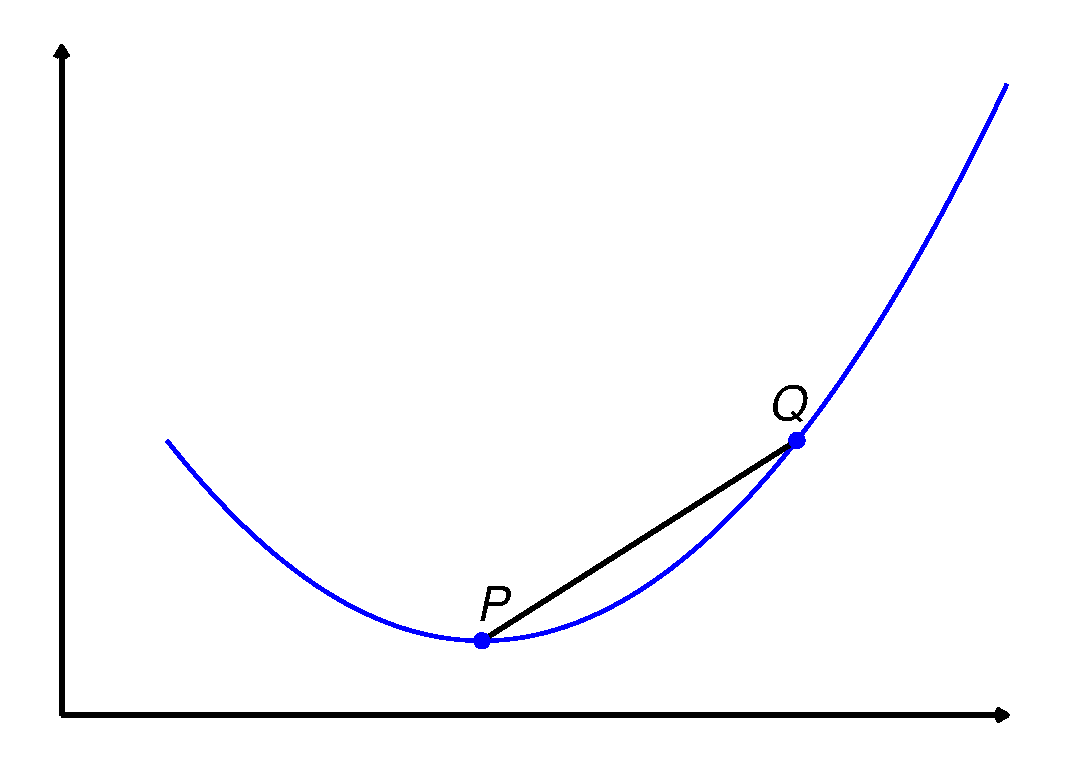
\includegraphics[width=15cm, height=7.9cm]{images/convexo.pdf}}
  \label{fig:convexo}
\end{figure}

\begin{definition}
	Una función $f: D \rightarrow \mathbb{R}$ es concava si $-f$ es convexa
\end{definition}

\begin{theorem}
	Sea $f$ definida en un punto $x_0$. Si $f$ tiene una derivada en $x_0$, entonces es continuo en $x_0$
\end{theorem}
\subsubsection{Demostración}
De la definición de derivada, se determina la siguiente igualdad
\begin{eqnarray}
	\phi(h) &=& \frac{f({x}_{0}+h)-f({x}_{0})}{h} \nonumber \\
	h \phi(h) &=& f({x}_{0}+h)-f({x}_{0}) \nonumber
\end{eqnarray}
Si existe la derivada de $f(x)$ en ${x}_{0}$, entonces $\phi(h) \rightarrow {f}^{'}({x}_{0})$ y como $h \rightarrow 0$ la expresión se desprende como
$$
f({x}_{0}+h) - f({x}_{0}) \rightarrow 0
$$
Por lo que para un determinado $\epsilon > 0$ existe un $\delta > 0$ tal que
$$
\lvert f({x}_{0}+h)-f({x}_{0}) \rvert < \epsilon
$$
Si $\lvert h \rvert < \delta$, se indica que $f(x)$ es continuo en ${x}_{0}$

%\begin{theorem}(\citep{Boyd_2004})
%	\label{convexo_dos_derivadas}
%	\begin{itemize}
%		\item[i] Si asumimos que $f$ es dos veces diferenciable, esto es la matriz Hessiana de segundo orden. Entonces $f$ es convexo si y solo si el dominio de $f$ es convexo y la matriz Hessiana es positiva semidefinida para todo $x \in dom(f)$
%		$$
%				{\nabla}^{2}f(x) \geq 0
%		$$
%		\item[ii] Si asumimos que $f$ es dos veces diferenciable, esto es la matriz Hessiana de segundo orden. Entonces $f$ es cóncavo si y solo si el dominio de $f$ es convexo y la matriz Hessiana es negativa semidefinida para todo $x \in dom(f)$
%		$$
%				{\nabla}^{2}f(x) \leq 0
%		$$
%	\end{itemize}
%\end{theorem}

\subsection{Máximo y mínimo de una función}
Para encontrar los máximos y mínimos de una función que sirve para hallar los valores óptimos, se debe encontrar los extremos de la función $f$ definida por $y=f(x)$ cuya derivada $f'(x)$ existe en cualquier conjunto abierto dentro de su dominio. \citep{Khuri_2002}

\begin{definition}
	Una función $f: D \rightarrow \mathbb{R}$ tiene un maximo local en un punto ${x}_{0} \in D$ si existe $\delta > 0$ tal que $f(x) \leq f({x}_{0})$ para todo $x \in {N}_{\delta}({x}_{0}) \cap D$. La función $f$ tiene un mínimo local en ${x}_{0}$ si $f(x) \geq f({x}_{0})$ para todo $x \in {N}_{\delta}({x}_{0}) \cap D$.
\end{definition}

\begin{definition}
	Una función $f: D \rightarrow \mathbb{R}$ tiene un máximo absoluto encima de $D$ si existe un punto $x^* \in D$ tal que $f(x) \leq f(x^*)$ para todo $x \in D$. La función $f$ tiene un mínimo absoluto encima de $D$ si existe un punto $x^* \in D$ tal que $f(x) \geq f(x^*)$ para todo $x \in D$.
\end{definition}

La determinación de los óptimos locales de $f$ son facilitados si $f$ es diferenciable

\begin{theorem}
	\label{teorema_min_max}
	Sea $f(x)$ diferenciable en un intervalo abierto $(a,b)$. Si $f(x)$ tiene un máximo o mínimo local en un punto ${x}_{0}$ en $(a,b)$, entonces $f'({x}_{0})=0$
\end{theorem}
\subsubsection{Demostración}
Suponga que $f$ tiene un máximo local en ${x}_{0}$. Entonces $f(x) \leq f({x}_{0})$ para todo $x$ en una vecindad ${N}_{\delta}({x}_{0}) \subset (a,b)$ resulta
\begin{equation}
	\frac{f(x)-f({x}_{0})}{x-{x}_{0}} =
	\left\{
	\begin{array}{ll}
		\leq 0, & \text{si } x > {x}_{0} \\
		\geq 0, & \text{si } x < {x}_{0}
	\end{array}
	\right.
\end{equation}
Para todo $x$ que pertenece a ${N}_{\delta}({x}_{0})$ como $x \rightarrow {x}_{0}^{+}$ la relación tendrá un límite no positivo, y si $x \rightarrow {x}_{0}^{-}$ la relación tendrá un límite no negativo. Mientras $f'(x_0)$ exista estos dos límites deben ser iguales a $f'({x}_{0})$ como $x \rightarrow {x}_{0}$ en lo que se concluye que $f'({x}_{0})=0$.

De igual forma suponga que $f(x)$ tiene un mínimo local en ${x}_{0}$. Entonces $f(x) \geq f({x}_{0})$ para todo $x$ en una vecindad ${N}_{\delta}({x}_{0}) \subset (a,b)$ resulta
\begin{equation}
	\frac{f(x)-f({x}_{0})}{x-{x}_{0}} =
	\left\{
	\begin{array}{ll}
		\geq 0, & \text{si } x > {x}_{0} \\
		\leq 0, & \text{si } x < {x}_{0}
	\end{array}
	\right.
\end{equation}
Para todo $x$ que pertenece a ${N}_{\delta}({x}_{0})$ como $x \rightarrow {x}_{0}^{+}$ la relación tendrá un límite no negativo, y si $x \rightarrow {x}_{0}^{-}$ la relación tendrá un límite no positivo. Mientras $f'(x_0)$ exista estos dos límites deben ser iguales a $f'({x}_{0})$ como $x \rightarrow {x}_{0}$ en lo que se concluye que $f'({x}_{0})=0$.

Una aplicación de la segunda derivada es la prueba para identificar valores máximos y mínimos locales como una consecuencia de la prueba de concavidad que sirve como alternativa a la primera prueba de la derivada \citep{stewart2016calculus}

\begin{itemize}
	\item \textbf{Prueba de la segunda derivada} Suponga que $f''$ es continuo cerca de un punto $c$.
	\begin{itemize}
		\item[\textbf{a)}] Si $f'(c)=0$ y $f''(c) > 0$, entonces $f$ tiene un mínimo local en $c$.
		\item[\textbf{b)}] Si $f'(c)=0$ y $f''(c) < 0$, entonces $f$ tiene un máximo local en $c$.
	\end{itemize}
\end{itemize}

\subsection{Variable aleatoria}
El concepto de variable aleatoria se define como una función del espacio muestral en el conjunto de números reales, esto permite considerar el resultado de un experimento aleatorio como un número real tomado por la variable aleatoria \citep{rincon2014introduccion}.

En general la variable aleatoria asigna un número real $x$ a cada elemento $e$ del espacio muestral $\Omega$. El dominio de $X$ es $\Omega$ y los números en el rango son números reales, en el cual la función $X$ se denomina variable aleatoria \citep{hines1988probabilidad}.

\begin{definition}
	Si $E$ es un experimento aleatorio que tiene espacio muestral $\Omega$, y $X$ es una función que asigna un número real $X(e)$ para todo resultado $e \in \Omega$, entonces $X(e)$ se llama variable aleatoria.
\end{definition}

\subsubsection{Función de distribución}
Por convención se utiliza una letra minúscula para denotar un valor particular de una variable aleatoria, del modo que $(X=x)$ es un evento del espacio del rango de la variable aleatoria $X$, donde $x$ es un número real. La probabilidad del evento $(X \leq x)$ puede expresarse como la función de $x$ en la siguiente forma
\begin{equation}
	F(x)=P(X \leq x)
\end{equation}
Donde $F(x)$ es llamada función de distribución, o función de distribución acumulativa de la variable aleatoria $X$

\subsection{Variable aleatoria discreta}\label{VADiscreta}
Generalmente estan relacionados al conteo, en el cual si $X$ es una variable aleatoria discreta, entonces $F(x)$ tendrá un número contablemente infinito de saltos y su rango $R=\{{x}_{1},{x}_{2},\ldots,{x}_{k},\ldots\}$
\begin{definition}\label{defn_vadisc}
	Si $X$ es una variable aleatoria discreta, asociamos un número\\ $p({x}_{i})=P(X={x}_{i})$ con cada resultado ${x}_{i}$, en $R$ para $i=1,2, \ldots , n, \ldots$ donde los números $p({x}_{i})$ satisfacen
	\begin{enumerate}
		\item $p({x}_{i}) \geq 0 \quad$ para todo $i$
		\item $\sum\limits_{i = 1}^{x}p({x}_{i})=1$ 
	\end{enumerate}
\end{definition}
En lo cual se observa que 
\begin{equation}
	\label{eq:prob:p_xi}
	p({x}_{i})=F({x}_{i})-F({x}_{i-1})
\end{equation}
y
\begin{equation}
	\label{eq:prob:p_xi2}
	F({x}_{i})=P(X \leq {x}_{i}) = \sum\limits_{x \leq {x}_{i}}^{}p(x)
\end{equation}
Empleando la ecuación (\ref{eq:prob:p_xi}) notamos el siguiente resultado para $b \geq a$
\begin{equation}
	P(a < X \leq b) = F(b) - F(a)
\end{equation}

\subsubsection{Esperanza}
Sea $X$ una variable aleatoria discreta con función de probabilidad $f(x)$. La esperanza de $X$ se define como el número
\begin{equation}
	E(X)=\sum\limits_{x}^{}xf(x)
\end{equation}

\subsubsection{Varianza}
Sea $X$ una variable aleatoria discreta con función de probabilidad $f(x)$. La varianza de $X$ se define como el número
\begin{equation}
	Var(X)=\sum\limits_{x}^{}{(x-\mu)}^{2}f(x)
\end{equation}
Donde $\mu$ es la esperanza de $X$ ($E[X]$) \citep{rincon2014introduccion}

\subsection{Variable aleatoria continua}\label{VAContinua}
En este caso se tiene un tramo continuo en los cuales el rango $R$ consistirá en uno o más intervalos, en la cual se define la función de densidad $f(x)$ como
\begin{equation}
	f(x) = \frac{d}{dx}F(x)
\end{equation}
y resulta que
\begin{equation}
	F(x) = \int_{- \infty}^{x}f(t)dt
\end{equation}
En la cual tiene la misma forma que (\ref{eq:prob:p_xi2}) reemplazando el simbolo de la sumatoria por la integral, entonces se tienen las siguientes propiedades de $f(x)$
\begin{enumerate}
	\item $f(x)\geq 0 \quad$ para todo $x \in {R}_{x}$
	\item $\int_{{R}_{x}}^{}f(x)dx=1$
	\item $f(x)$ es un tramo continuo.
	\item $F(x)=0$ si $x \notin {R}_{x}$ 
\end{enumerate}
De la misma forma en un rango para $x$ la función $f$ es estable si cumple lo siguiente
\begin{equation}
	P\{ e \in \Omega: a \leq X(e) \leq b \} = \int_{b}^{a}f(x)dx
\end{equation}
\citep{hines1988probabilidad}

\subsubsection{Esperanza}
Sea $X$ una variable aleatoria continua con función de densidad $f(x)$, la esperanza esta definida como
\begin{equation}
	E(X) = \int_{- \infty}^{\infty} xf(x)dx
\end{equation}
Suponiendo que esta integral es absolutamente convergente, es decir, cuando la integral de los valores absolutos es convergente.

\subsubsection{Varianza}
Sea $X$ una variable aleatoria continua con función de densidad $f(x)$. La varianza de $X$ se define como el número
\begin{equation}
	Var(X)= \int_{- \infty}^{\infty} {(x-\mu)}^{2} f(x)dx
\end{equation}
Donde $\mu$ es la esperanza de $X$ ($E[X]$), además de que esta integral debe ser convergente \citep{rincon2014introduccion}.

\subsection{Distribución normal}\label{Dist_normal}
La distribución normal es de las más importantes tanto en la parte teórica como la aplicativa de la estadística \citep{hines1988probabilidad}. Se afirma que una variable aleatoria $X$ tiene una distribución normal con media $\mu (- \infty < \mu < \infty)$ y varianza ${\sigma}^{2} > 0$ y tiene la función de densidad
\begin{equation}
	\label{distribucion_normal}
	f(x) = \frac{1}{\sigma \sqrt{2 \pi}} {e}^{-\frac{1}{2} {\left( \frac{x- \mu}{\sigma} \right)}^{2}}
\end{equation}

Con media $\mu$ y varianza ${\sigma}^{2}$. Su notación abreviada es $X \sim N(\mu, {\sigma}^{2})$ para indicar que la variable aleatoria $X$ se distribuye normalmente con media $\mu$ y varianza ${\sigma}^{2}$.

\subsubsection{Distribución normal acumulativa}
La función de distribución acumulativa $F$ es
\begin{equation}
	F(x) = P(X \leq x) = \int_{-\infty}^{x} \frac{1}{\sigma \sqrt{2 \pi}} {e}^{-\frac{1}{2} {\left( \frac{x- \mu}{\sigma} \right)}^{2}} d \mu
\end{equation}
La evaluación de la integral es muy complicado, por lo que es necesario aplicar métodos numéricos. Sin embargo una transformación de variables $z = \frac{x-\mu}{\sigma}$, permite que la evaluación sea independiente de $\mu$ y $\sigma$. de la siguiente forma
\begin{eqnarray}
	F(x) &=& P(X \leq x) = P \left( Z \leq \frac{x-\mu}{\sigma} \right) \nonumber \\
	F(x) &=& \int_{- \infty}^{(x-\mu) / \sigma} \frac{1}{\sqrt{2 \pi}} {e}^{- \frac{{z}^{2}}{2}}dz \nonumber \\
	\label{distribucion_normal_acum}
	F(x) &=& \int_{- \infty}^{(x - \mu)/ \sigma} \varphi (z)dz \nonumber \\
	F(x) &=& \Phi \left( \frac{x-\mu}{\sigma} \right)
\end{eqnarray}

\subsubsection{Distribución normal estándar}
De la distribución de probabilidad en (\ref{distribucion_normal_acum}) se tiene
\begin{equation}
	\varphi (z) = \frac{1}{\sqrt{2 \pi}} {e}^{- \frac{{z}^{2}}{2}} \quad -\infty < z < \infty
\end{equation}
Es una distribución normal con media $0$ y varianza $1$, esto indica que $Z \sim N(0,1)$ en la cual $Z$ es una \textsl{distribución normal estándar}, su gráfica de función de densidad se muestra en la Figura \ref{fig:norm_z}.
\begin{figure}[H]
  \caption{Distribución normal estándar $Z \sim N(0,1)$}
  {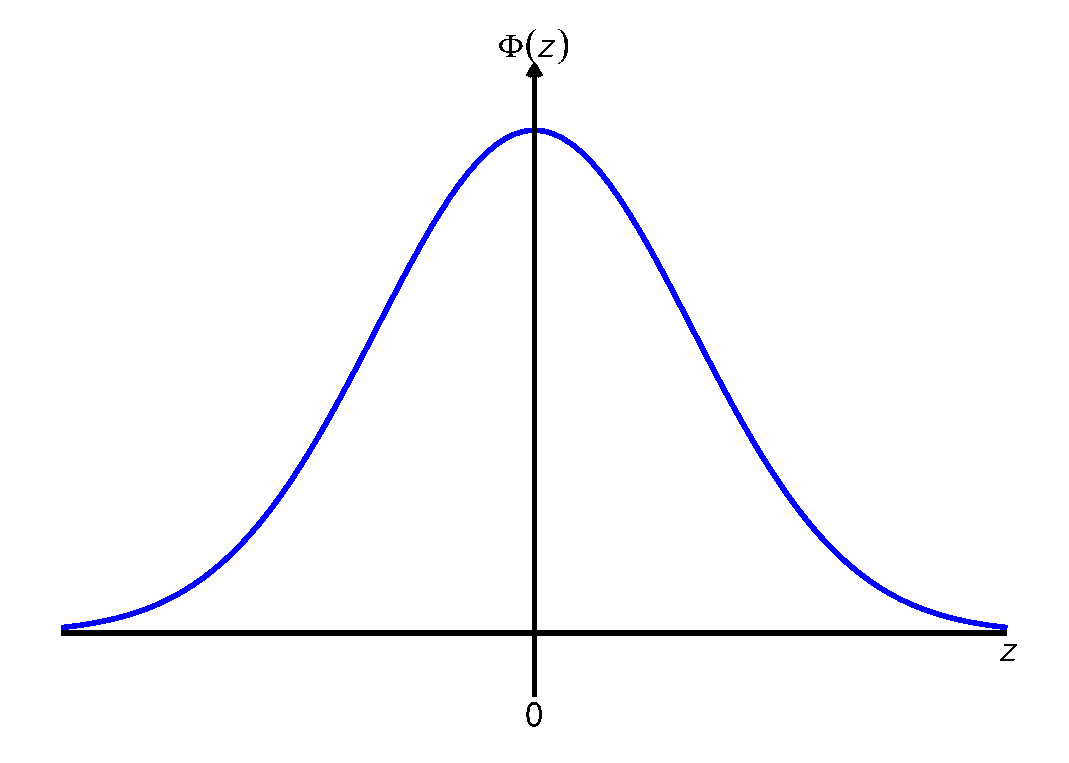
\includegraphics[width=15cm, height=7.9cm]{images/norm_estn.pdf}}
  \label{fig:norm_z}
\end{figure}

La función de distribución correspondiente ahora es $\Phi$
\begin{equation}
	\Phi (z) = \int_{-\infty}^{z} \frac{1}{\sqrt{2 \pi}} {e}^{- \frac{{z}^{2}}{2}} dz
\end{equation}

\subsection{Costos}
La contabilidad de costos determina el costo estimado hacia el real del producto o servicio para valorarlo y considerarlo en su precio de venta. La gestión de costos es la actividad de medición y análisis. \citep{toomey2000inventory}

Los costos deben considerar tanto los costos directos e indirectos, como por ejemplo el costo directo viene a ser el costo de compra mientras que los costos indirectos viene a ser los gastos generales de fabricación y materiales. \cite{haeussler2003matematicas} indican que el \textsl{costo fijo} es la suma de costos independientes del nivel de producción como renta, seguros entre otros; mientras que el \textsl{costo variable} es la suma de todos los costos dependientes del nivel de producción como salarios y materiales. De esta forma el \textsl{costo total} es la suma de los costos variables y fijos.

\newpage
\subsection{Clasificación de actividades basada en costos (ABC)}
\label{section:ABC}
\cite{toomey2000inventory} lo indica como un modo alternativo a la gestión de costos en el cual se acumulan los costos de los productos o servicios brindados de tal forma que clasifica los trabajos en base a sus costos acumulados, en lugar de categorías contables que permita una gestión de costos efectiva. Su propósito es dividir todos los productos o articulos que se tienen en el inventario y clasificarlas en tres grupos (A, B y C), en el cual se le debe dedicar más tiempo a la administración a los productos que representan el mayor costo monetario \citep{render2006metodos}.

La clasificación de los productos son descritos a continuación:
\begin{enumerate}
	\item \textbf{Grupo A:} Son los productos que poseen la mayor parte de los costos de todo el inventario que suele conformar el $70\%$, sus niveles de inventario deben ser monitoreados con una prioridad alta aunque estos solo comprendan el $10\%$ de todos los artículos del inventario, siendo así su tiempo de dedicación no muy alto.
	\item \textbf{Grupo B:} Son los productos que poseen costos moderados de todo el inventario conformando el $20\%$ siendo menores a los del grupo A, sus productos comprenden también el $20\%$ de todos los artículos del inventario, por lo cual su tiempo de dedicación debería ser menor a los del grupo A, especialmente a los costos más altos del grupo B.
	\item \textbf{Grupo C:} Son los productos que poseen la menor cantidad de costos del inventario conformando solo el $10\%$, aunque sus productos comprenden el $70\%$ de todo el inventario. Para este grupo no es beneficioso dedicar mucho tiempo a la administración de sus artículos como a los de grupo A y B.
\end{enumerate} 
La Tabla \ref{table:ABC_resumen} resume el análisis ABC.
\begin{table}[h!]
    \caption{Resumen de actividades basadas en costos (ABC)}
    \begin{tabular}{p{0.8cm} p{2.52cm} p{5.2cm} p{4.9cm}} % Define anchos personalizados para cada columna
        \hline
        \textbf{Grupo} & \textbf{$(\%)$ de Costos} & \textbf{$(\%)$ ocupación del inventario} & \textbf{Usar técnicas cuantitativas} \\
        \hline
        \textbf{A} & $70\%$ & $10\%$ & Si \\
        \textbf{B} & $20\%$ & $20\%$ & Los que tienen costos altos \\
        \textbf{C} & $10\%$ & $70\%$ & No \\
        \hline
    \end{tabular}
    \label{table:ABC_resumen}
\end{table}


\subsection{Inventarios}
La sociedad estadounidense de producción e inventario (APICS) lo define como la rama de la gestión empresarial que se ocupa de la planificación y el control de inventarios, en el cual su función es mantener un nivel de existencias deseado de productos o artículos específicos. \citep{toomey2000inventory}

El rol principal del inventario es servir o brindar servicio al cliente, esto implica factores como la disponibilidad de la cantidad pedida, momento correcto, lugar correcto y costo correcto. Su objetivo principal es minimizar las inversiones en inventarios y al mismo tiempo cumplir con los requisitos funcionales sin alterar las operaciones normales.

Un sistema que controla los inventarios tiene que ser compatible con los objetivos, funciones y demandas del inventario en particular.

\subsection{Modelos de inventarios}

%\subsection{Modelo General de Inventario}

Los problemas de inventarios son relacionados sobre reservas de cierto artículo o insumo utilizado para satisfacer las demandas. Por lo cual el exceso de existencias provoca un mayor costo de capital y almacenamiento, mientras que el desabesticimiento interrumpe las producciones y/o las ventas. En el que se debe optimizar el nivel de inventario que equilibre las dos situaciones minimizando una función de costo apropiada. Esto se define en diseñar una \textsl{política de inventario} \citep{taha2012investigacion} que responda las preguntas:

\begin{enumerate}
	\item ¿Cuánto pedir?
	\item ¿Cuándo pedir?
\end{enumerate}

En la cual su base del modelo de inventario es la siguiente función de costo genérica para el costo total del inventario $CTI(y)$

$$
\begin{pmatrix}
\text{Costo total del} \\ 
\text{inventario}
\end{pmatrix}
=
\begin{pmatrix}
\text{Costo de} \\ 
\text{compra}
\end{pmatrix}
+
\begin{pmatrix}
\text{Costo de} \\ 
\text{preparación}
\end{pmatrix}
+
\begin{pmatrix}
\text{Costo de} \\ 
\text{retención}
\end{pmatrix}
+
\begin{pmatrix}
\text{Costo por} \\ 
\text{escasez}
\end{pmatrix}
$$

Donde:

\begin{enumerate}
	\item \textbf{Costo de compra $(C)$: }Es el costo por unidad de un artículo de inventario. Puede haber momentos en que el artículo se ofrece con descuento si el tamaño del pedido excede una cantidad determinada, lo cual es un factor importante a tomar en cuenta al momento de tomar la decisión de \textsl{cuánto pedir}.

	\item \textbf{Costo de preparación $(K)$: }Representa los costos que incurren cuando se coloca un pedido, es decir los costos que llevan la elaboración o brindación del servicio o su producto independientemente de su tamaño.

	\item \textbf{Costo de retención (almacenamiento) $(h)$: }Representa el costo de mantener las existencias de productos sobrantes. Estos costos incluyen el interés sobre el capital y el costo de almacenamiento, mantenimiento y manejo del producto.

	\item \textbf{Costo por escasez (faltante) $(p)$: }Este costo es tomado como una penalización en que se incurre cuando se agotan las existencias. Incluye la pérdida potencial de ingresos, la interrupción de la producción y el costo subjetivo de pérdida de lealtad del cliente debido a la falta del producto.
\end{enumerate}

Esto también puede expresarse de la siguiente manera:
\begin{equation}
	\label{2.1}
	CTI(y) = C + K + h + p
\end{equation}

\subsection{Política sobre un modelo de inventarios}

Entonces se hacen las siguientes preguntas sobre cuando y cuanto debe reabastecerse un inventario. Por el cual la administración científica de inventarios debe comprender los siguientes pasos:
\begin{enumerate}
	\item Plantear un \textsl{modelo matemático} que describa el comportamiento del sistema de inventarios.
	\item Elaborar una política óptima de inventarios a partir del modelo.
	\item Utilizar un \textsl{sistema de procesamiento de información computarizado} para mantener registros de los niveles del inventario.
	\item A partir de estos registros, utilizar la política óptima de inventarios para señalar cuándo y cuánto conviene reabastecer. 
\end{enumerate}

Los modelos matemáticos de inventarios que se utilizan bajo estos pasos son los modelos determinísticos y estocásticos, el modelo dependerá según la posibilidad de predecir la demanda. \citep{hillier2003introduccion}

\subsection{Clasificación de un sistema de inventarios}

Asimismo un sistema de inventario puede requerir \textsl{revisiones periódicas} es decir en un cierto intervalo de tiempo como una semana o cada mes. De forma alterna puede estar basado en \textsl{revisiones continuas}, que es cuando se realiza un pedido cuando el nivel del inventario se reduce a un punto de volver a pedir o \textsl{punto de reorden (R)}.

\subsection{Demanda}
La complejidad de los modelos de inventario depende de si la demanda ($D$) es determinística o probabilística, además que esta pueda variar con el tiempo. \citep{hillier2003introduccion}

Cuando se tiene una demanda determinística se conocen los pedidos siguientes, asimismo sobre intervalos de tiempos iguales la demanda puede ser constante (estática) o variable (dinámica).

En el caso de una demanda probabilística se efectúa cuando la demanda en un periodo de tiempo es incierta, pero puede describirse en términos de una distribución de probabilidad, en el caso de las demandas probabilísticas se tienen que estas puedan ser estacionarias o no estacionarias sobre el tiempo.

%De forma general el patrón de la demanda en un modelo de inventario puede asumir uno de estos tipos:
%\begin{enumerate}
%	\item Determinístico y constante (estático) con el tiempo.
%	\item Determinístico y variable (dinámico) con el tiempo.
%	\item Probabilístico y estacionario a lo largo del tiempo.
%	\item Probabilístico y no estacionario a lo largo del tiempo. 
%\end{enumerate}

Entonces para seleccionar el modelo de inventario, debemos determinar si se va a utilizar un modelo determinístico o probabilístico. Esta decisión es más factible calculando el \textsl{coeficiente de variabilidad} $(CV)$ tomando los siguientes pasos
\begin{enumerate}
	\item Calcular la demanda promedio en el periodo evaluado es decir tomar la \textsl{Media}.
	$$
	\textsl{Media}=\frac{1}{n}\sum\limits_{i = 1}^{n}{d}_{i}
	$$
	\item Encontrar una estimación de la varianza de la demanda por periodo, es decir tomar la \textsl{Varianza}.
	$$
	\textsl{Varianza}=\frac{1}{n}\sum\limits_{i = 1}^{n}{(d_i-\textsl{Media})}^2
	$$
	\item Determinar el coeficiente de variabilidad ($CV$) que representa la variabilidad relativa de la demanda con la siguiente fórmula
	\begin{equation}
	\label{CVar}
	CV = \frac{\textsl{Varianza}}{\textsl{Media}^2}
\end{equation}
	\item Si el ($CV$) (\ref{CVar}) es menor a 0.20, indica que la demanda es relativamente estable en los periodos evaluados, y por lo tanto tiene una demanda determinística. Si resulta mayor o igual a 0.20 indica que la demanda no es estable y además, por lo que posee una demanda probabilística.
\end{enumerate}


%\subsection{Multiplicadores de Lagrange}
%Un importante teorema que ayuda en funciones restringidas es el de ``Multiplicadores de Lagrange'' formulada por Joseph-Louis Lagrange, más conocido como Giuseppe Luigi Lagrangia, quien fue un físico, matemático y astrónomo italiano nacido en Turín el 25 de enero de 1736. Además de sus principales logros fue demostrar el teorema del valor medio, desarrollar la mecánica Lagrangiana y su importante contribución en astronomía. Falleciendo en Paris el 10 de abril de 1813. \citep{cardenascalculo}

\subsection{Modelos de inventario determinísticos}

Este modelo asume que la demanda y el tiempo de entrega son conocidos y fijos, adicionalmente en los modelos estáticos se tiene una demanda constante en función del tiempo. \citep{taha2012investigacion}

\manualsubsubsection{2.2.15.1}{Modelo clásico de cantidad económica de pedido (EOQ)}\label{Modelo_clas_EOQ}
La abreviación EOQ proviene del inglés (economic order quantity) que significa cantidad económica pedido. Este primer modelo asume que la demanda es constante y las ordenes llegan en el momento que se están solicitando. Se basa en los siguientes supuestos:
\begin{enumerate}
	\item Tasa de demanda conocida por unidad de tiempo.
	\item La cantidad ordenada de inventario llega cuando se desea, indicando un tiempo de espera igual a cero.
	\item No se tienen faltantes.
\end{enumerate}
\clearpage
Como la demanda es constante a través de los intervalos de tiempo, se tiene un inventario disminuido con comportamiento uniforme, de tal forma que cuando el inventario llega a una cantidad nula o cero, con el nuevo pedido este nivel de inventario debe incrementarse a ``$y$'' unidades. El proceso continuará con esta conducta a través del tiempo.

Según al modelo se definen las siguientes componentes:

\begin{itemize}
	\item[$y=$] Cantidad de pedido, que viene a ser el número de unidades pedidas.
	\item[$D=$] Tasa de demanda, expresado en las unidades de medidas sobre el tiempo evaluado.
	\item[$T=$] Duración del ciclo de pedido, expresado en el tiempo evaluado desde el momento que se tiene el pedido hasta el siguiente pedido.
\end{itemize}

Gráficamente se puede observar en la Figura \ref{fig:img1} la conducta del modelo clásico de cantidad económica de pedido.

\begin{figure}[H] %Colocar H mayuscula en lugar del h!
  \caption{Conducta de inventario en el modelo clásico económica de pedido (EOQ)}
  {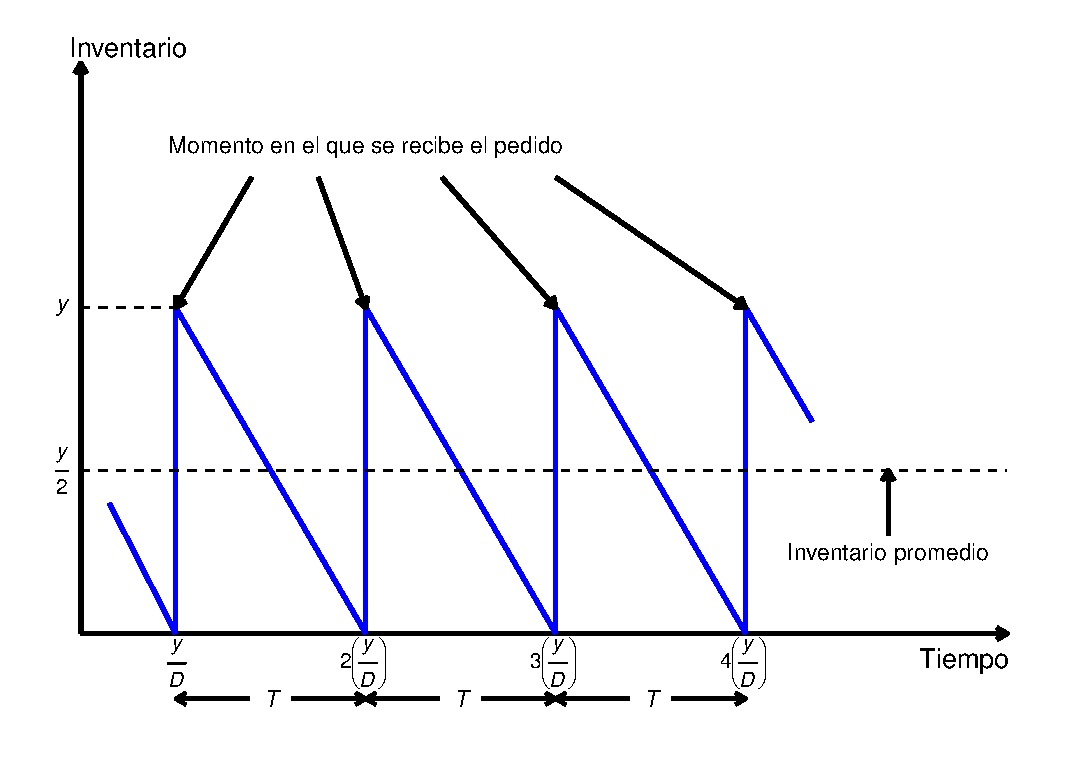
\includegraphics[width=15cm, height=8.5cm]{images/img1.pdf}}
  \label{fig:img1}
\end{figure}

Durante los pedidos, se tiene un intervalo de tiempo que comienza con el abastecimiento del pedido y culmina en el punto en el que se recibe el siguiente abastecimiento del pedido, por tanto se tiene la siguiente relación
\begin{equation}
	\label{T}
	T = \frac{y}{D}
\end{equation}

Para el modelo de costos del modelo EOQ se requieren dos parámetros esenciales
\begin{itemize}
	\item[$K=$] Costo de preparación del pedido
	\item[$h=$] Costo de retención
\end{itemize}

El nivel de inventario promedio ($NIP$) que se mide en unidades sobre el tiempo se encuentra expresado de la siguiente forma:
\begin{equation}
	\label{NIP}
	NIP=\frac{y}{2}
\end{equation}

El costo de almacenamiento por unidad de tiempo ($CAT$) estaría en función del costo de almacenamiento $h$ por el nivel promedio de inventario $(NIP)$ expresado en la ecuación (\ref{NIP}):
\begin{eqnarray}
	\label{CAT}
	CAT &=& h(NIP) \nonumber \\
	CAT &=& h\left(\frac{y}{2} \right)
\end{eqnarray}
Entonces el costo de almacenamiento por intervalo de tiempo ($CAIT$) vendría a estar expresado como el producto del tiempo entre abastecimientos del producto por el costo de almacenamiento por unidad de tiempo, de la siguiente forma:
\begin{eqnarray}
	CAIT = T * CAT \nonumber
\end{eqnarray}
Reemplazando los valores por las expresiones (\ref{T}) y (\ref{CAT}) se tiene la siguiente expresión para el costo de almacenamiento por intervalo de tiempo 
\begin{eqnarray}
	\label{CAIT}
	CAIT &=&  \left( \frac{y}{D} \right)  \left[ h \left( \frac{y}{2} \right) \right]  \nonumber \\
	CAIT &=& \frac{h {y}^{2}}{2D}
\end{eqnarray}
Ahora el costo por cada orden realizada o costo por la producción en el intervalo de tiempo ($CPT$) estaría expresado como:
\begin{equation}
	\label{CPT}
	CPT = K + Cy
\end{equation}
De lo que el costo total por intervalo de tiempo ($CTT$) sería el costo de almacenamiento por intervalo de tiempo (\ref{CAIT}) más el costo de producción por intervalo de tiempo (\ref{CPT})
\begin{eqnarray}
	\label{CTT}
	CTT &=& CAIT + CPT \nonumber \\
	CTT &=& \frac{h {y}^{2}}{2D} + K + Cy
\end{eqnarray}
Si al costo total por intervalo de tiempo ($CTT$) de la expresión (\ref{CTT}) lo dividimos entre el tiempo $T$, se tendría el costo total del inventario ($CTI$)
\begin{eqnarray}
	\label{CTIdejado}
	CTI(y) = \frac{CTT}{T} 
\end{eqnarray}
Reemplazando por los valores de la ecuación (\ref{CTT}) y (\ref{T}) se tiene la siguiente expresión para el costo total del inventario del modelo EOQ
\begin{eqnarray}
	\label{CTI}
	CTI(y) &=& \frac{\frac{h {y}^{2}}{2D} + K + Cy}{\frac{y}{D}} \nonumber \\
	CTI(y) &=& \frac{KD}{y} + DC + \frac{hy}{2}
\end{eqnarray}
De donde se tiene las siguientes componentes
\begin{itemize}
	\item[$\frac{KD}{y}$:] Costo de preparación de pedidos expresado como el costo por pedido multiplicado por el número de pedidos.
	\item[$DC$:] Costo de aprovisionamiento sirve para satisfacer toda la demanda, ya que no se permiten faltantes. Esta en función del producto entre los costos por unidad y la demanda.
	\item[$\frac{hy}{2}$:] Costo de almacenamiento por unidad de tiempo ($CAT$) expresado en (\ref{CAT}).
\end{itemize}	
Se debe minimizar el costo total de inventario $CTI(y)$, en la ecuación (\ref{CTI}) se observa que el $CTI(y)$ esta en función del costo por ordenar y el costo por almacenar.
En todo caso se tiene que minimizar la suma del costo por ordenar y el costo por almacenar, de tal forma que se minimice el costo total de inventario. El valor óptimo de cuanto pedir ``$y$'' es minimizando el $CTI(y)$ mediante la derivación e igualando a cero teniendo como se demostró en el Teorema $\ref{teorema_min_max}$:
\clearpage
\begin{eqnarray}
	\label{dCTI}
	\frac{dCTI(y)}{dy} &=& 0 \nonumber \\
	\frac{dCTI(y)}{dy} &=& \frac{d}{dy}\left(\frac{KD}{y} + DC + \frac{hy}{2} \right) = 0 \nonumber \\
	\frac{dCTI(y)}{dy} &=& - \frac{KD}{y^2} + \frac{h}{2} = 0
\end{eqnarray}
Despejando ``$y$'' en la ecuación (\ref{dCTI}) se obtiene la cantidad de pedido óptima $y^*$ de la siguiente manera
\begin{eqnarray}
	\label{yopt}
	\frac{h}{2} &=& \frac{KD}{y^2} \nonumber \\
	y^2 &=& \frac{2KD}{h} \nonumber \\
	y &=& \pm \sqrt{\frac{2KD}{h}} \qquad \text{(solo se considera la parte positiva)} \nonumber \\
	y^* &=& \sqrt{\frac{2KD}{h}}
\end{eqnarray}
Asimismo la cantidad de pedido es mínima mediante la prueba de la segunda derivada.
\begin{eqnarray}
	\label{minimo1}
	\frac{d^2 CTI(y)}{dy^2} &=& \frac{d^2}{dy^2} \left(\frac{KD}{y} + DC + \frac{hy}{2} \right) \nonumber \\
	\frac{d^2 CTI(y)}{dy^2} &=& \frac{2KD}{y^3} \geq 0; \quad \forall y > 0
\end{eqnarray}
Ahora tomando la ecuación del ciclo de pedido $T$ (\ref{T}) y la cantidad de pedido óptima $y^*$  (\ref{yopt}) se tiene la respuesta a cuando pedir o el intervalo de pedido óptimo $T^*$
%\newpage
\begin{eqnarray}
	\label{Topt}
	T &=& \frac{y}{D} \nonumber \\
	T^* &=& \frac{y^*}{D} \nonumber \\
	T^* &=& \frac{\sqrt{\frac{2KD}{h}}}{D} \nonumber \\
	T^* &=& \sqrt{\frac{2K}{Dh}}
\end{eqnarray}
De la misma forma tomando la ecuación de costo total de inventario $CTI(y)$ (\ref{CTI}) reemplazando con los valores de la cantidad de pedido óptima $y^*$ (\ref{yopt}) se obtiene el costo mínimo total de inventario óptimo $CTI(y^*)$
\begin{eqnarray}
	\label{CTIopt}
	CTI(y) &=& \frac{KD}{y} + DC + \frac{hy}{2} \nonumber \\
	CTI(y^*) &=& \frac{KD}{y^*} + DC + \frac{hy^*}{2} \nonumber \\
%\end{eqnarray}
%Ahora reemplanzando $y^*$ por los valores de (\ref{yopt} se tiene
%\begin{eqnarray}
	CTI(y^*) &=& \frac{KD}{\sqrt{\frac{2KD}{h}}} + DC + \frac{h \left( \sqrt{\frac{2KD}{h}} \right)}{2} \nonumber \\ 
	CTI(y^*) &=& KD \sqrt{\frac{h}{2KD}} + DC + \sqrt{\frac{hKD}{2}} \nonumber \\
	CTI(y^*) &=& \sqrt{\frac{hKD}{2}} + DC + \sqrt{\frac{hKD}{2}} \nonumber \\
	CTI(y^*) &=& 2 \sqrt{\frac{hKD}{2}} + DC \nonumber \\
	CTI(y^*) &=& \sqrt{2hKD} + DC
\end{eqnarray}
Generalmente los pedidos no llegan en el mismo momento que se hace la solicitud de pedido, lo que sucede es un tiempo de espera o tiempo de entrega, que depende a la frecuencia del tiempo ya sean días o hasta semanas. Por lo cual el inventario de igual forma tiene que estar disponible para la demanda una vez ya realizada el pedido. Entonces la decisión de cuándo ordenar es conocida como punto de reorden ($R$) esto se observa en la Figura \ref{fig:img2}.
\begin{figure}[H]
  \caption{Punto de reorden ($R$) del modelo (EOQ)}
  {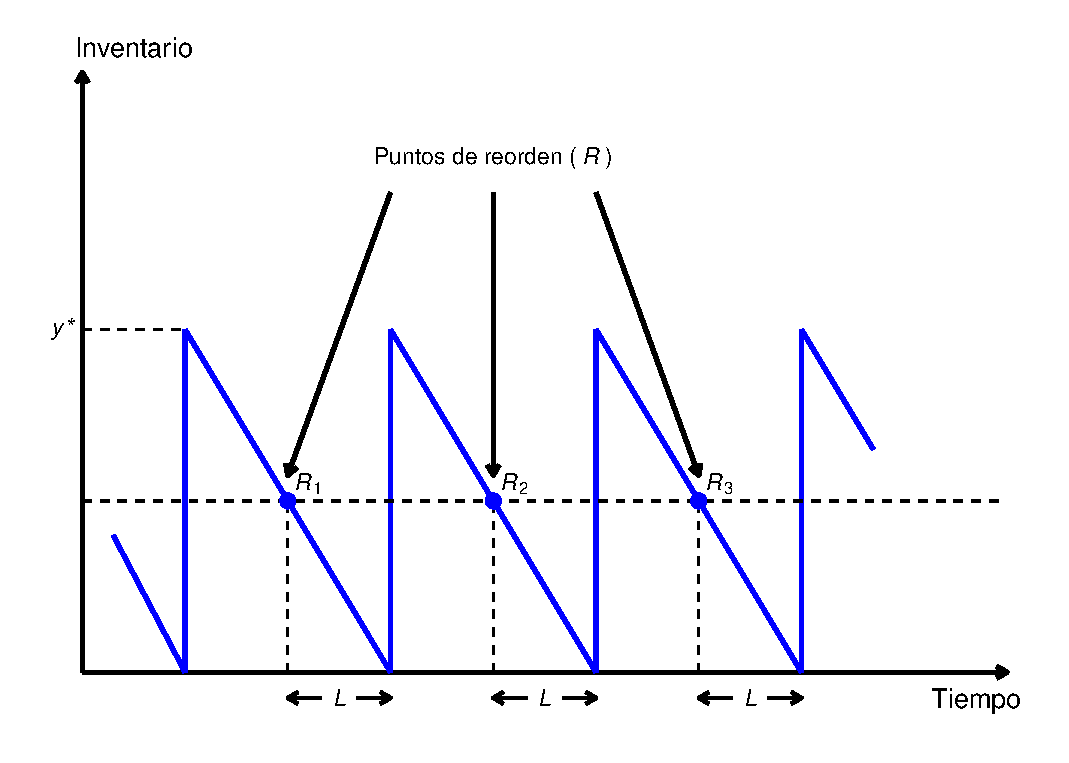
\includegraphics[width=15cm, height=6.5cm]{images/img2.pdf}}
  \label{fig:img2}
\end{figure}

Donde se observa que el punto de reorden se establece tomando en cuenta los siguientes casos. Sea $L$ el tiempo de entrega, entonces el punto de reorden $R$ es:
\begin{itemize}
	\item $R = LD$, si $L < T^*$ es decir que la demanda durante el tiempo de entrega es menor a la cantidad óptima $y^*$, en el cual el punto de reorden es la demanda por el tiempo de entrega.
	\item $L_e = L - nT^*$, si $L > T^*$ es decir que la demanda durante el tiempo de entrega es mayor que la cantidad óptima $y^*$, en el cual el pedido debe realizarse en el periodo del pedido anterior. Por lo que el punto de reorden vuelve a ser
\end{itemize}
$$
	R = L_e D
$$
Por lo cual enunciamos lo siguiente: \textsl{``Pedir la cantidad $y^*$ siempre que el nivel de inventario se reduzca $L_e D$ unidades''}.

\manualsubsubsection{2.2.15.2}{Modelo clásico de cantidad económica de pedido (EOQ) con descuentos}
Algo más general del modelo EOQ es que el precio del producto del inventario  varíe con la cantidad que se compre o produzca. Es decir que se puede obtener un descuento si el tamaño del pedido ``$y$'' excede un límite ``$q$'' establecido. Por lo cual se tiene un precio unitario de compra ``$c$'', expresado de la siguiente manera:
\begin{equation}
	\label{c_descuento}
	c =
	\left\{
	\begin{array}{ll}
		c_1, & \text{si } y \leq q \\
		c_2, & \text{si } y > q
	\end{array}
	\right\}, \quad c_1 > c_2
\end{equation}
De tal forma que el costo de compra por intervalo de tiempo ($CCIT$) estaría en función del precio unitario de compra ``$c$'' (\ref{c_descuento}) y el tiempo de pedido ``$T$'' (\ref{T}), quedando de la siguiente manera
\begin{equation}
	CCIT = \left\{%
	\begin{array}{ll}
		\frac{c_1 y}{T} = \frac{c_1 y}{\left( \frac{y}{D} \right)} = Dc_1 , & y \leq q \\ 
		\frac{c_2 y}{T} = \frac{c_2 y}{\left( \frac{y}{D} \right)} = Dc_2 , & y > q 
	\end{array}%
	\right.
\end{equation}
\clearpage
\noindent Asi mismo si aplicamos la notación utilizada con el precio de compra ``$c$'' (\ref{c_descuento}) en (\ref{CTI}), el costo total de inventario $CTI(y)$ estaría expresado de la siguiente manera
\begin{equation}
	\label{CTI_descuento}
	CTI(y) = \left\{%
	\begin{array}{ll}
		CTI_1 (y) = Dc_1 + \frac{KD}{y} + \frac{hy}{2} , & y \leq q \\ 
		CTI_2 (y) = Dc_2 + \frac{KD}{y} + \frac{hy}{2} , & y > q 
	\end{array}%
	\right.
\end{equation}
En la ecuación (\ref{CTI_descuento}) se observa que $c_i,$ donde $i = \{ 1,2 \}$ actúa como constante si es que deseamos minimizar ``$y$'', e igualar a cero obteniedo nuestra cantidad de pedido óptima $y^*$ tal como se realizó en la expresión (\ref{yopt}) y el Teorema (\ref{teorema_min_max}). Entonces la cantidad óptima de pedido con descuentos $y_m$ es igual a
\begin{equation}
	y_m = \sqrt{\frac{2KD}{h}}
\end{equation}
El costo se ve ilustrado en la Figura \ref{fig:img3}.

\begin{figure}[H]
  \caption{Función de costos de inventario con descuentos en el precio}
  {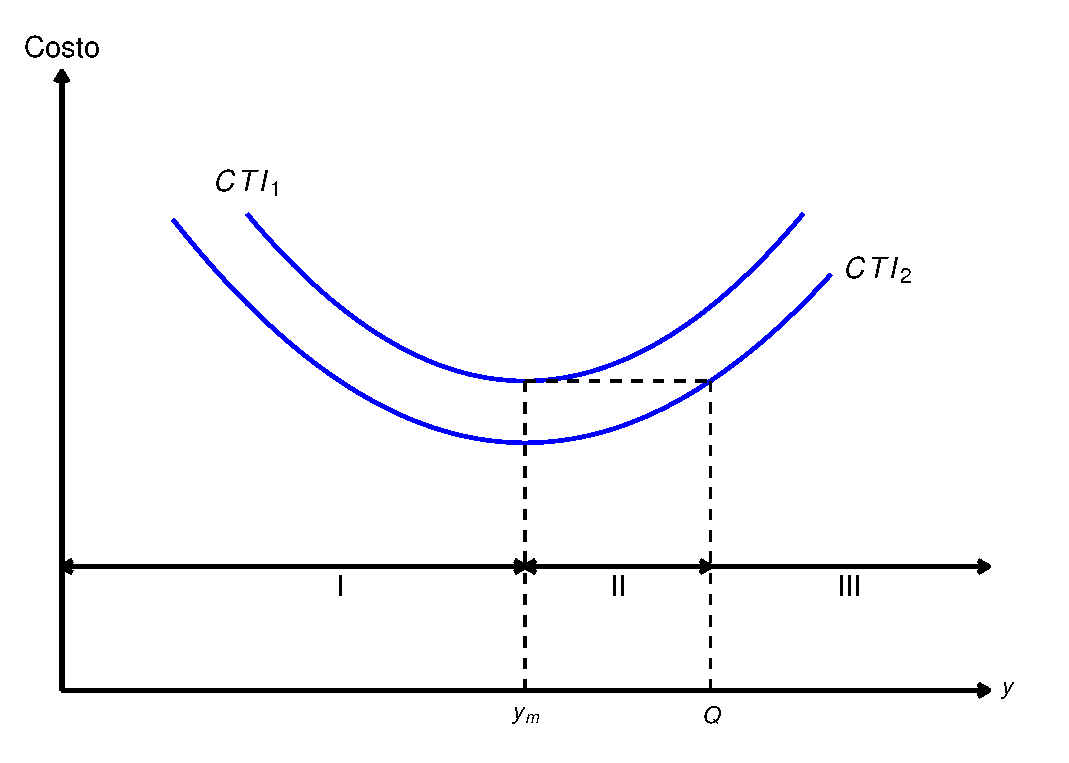
\includegraphics[width=15cm, height=8cm]{images/img3.pdf}}
  \label{fig:img3}
\end{figure} 
En donde la determinación de la cantidad de pedido óptima $y^*$ sera de acuerdo al punto de discontinuidad de precio $q$, con respecto a las zonas I, II y III, limitadas por los intervalos:

\begin{itemize}
	\item \textbf{ZONA I:} en el intervalo $(0, y_m)$
	\item \textbf{ZONA II:} en el intervalo $(y_m, Q)$
	\item \textbf{ZONA III:} en el intervalo $(Q, \infty)$
\end{itemize}

El valor de $Q (> y_m)$ se determina mediante la siguiente ecuación
$$
CTI_2 (Q) = CTI_1 (Q)
$$
Reemplazando $CTI_2 (Q)$ por los valores de la expresión (\ref{CTI_descuento}) se tiene
\begin{eqnarray}
	Dc_2 + \frac{KD}{Q} + \frac{hQ}{2} &=& CTI_1 (Q) \nonumber \\
	\frac{2QDc_2 + 2KD + hQ^2}{2Q} &=& CTI_1 (y_m) \nonumber \\
	2QDc_2 + 2KD + hQ^2 - 2Q [ CTI_1 (ym) ] &=& 0 \nonumber
\end{eqnarray}
A la expresión lo dividimos por el costo de almacenamiento $h \neq 0$ el cual se simplifica en
\begin{eqnarray}
	\label{Q_descuento}
	\frac{2QDc_2 + 2KD + hQ^2 - 2Q [ CTI_1 (ym) ]}{h} &=& \frac{0}{h} \nonumber \\
	\frac{2QDc_2}{h} + \frac{2KD}{h} + \frac{hQ^2}{h} - \frac{2Q [ CTI_1 (y_m) ]}{h} &=& 0 \nonumber \\
	Q^2 + \frac{2QDc_2}{h} - \frac{2Q [ CTI_1 (y_m) ]}{h} + \frac{2KD}{h} &=& 0 \nonumber \\
	Q^2 + \left( \frac{2[ Dc_2 - CTI_1 (y_m) ]}{h} \right) Q + \frac{2KD}{h} &=& 0 
\end{eqnarray}
En la Figura \ref{fig:img4} se muestra la cantidad óptima deseada $y^*$ en base a la zona que se encuentre $q$.
En el cual se observa que la cantidad óptima $y^*$ que se busca es
\begin{equation}
	\label{CTI_descuento2}
	y^* = \left\{%
	\begin{array}{ll}
		y_m & \text{, si } q \text{ se encuentra en las zonas I o III} \\ 
		q & \text{, si } q \text{ se encuentra en la zona II}
	\end{array}%
	\right.
\end{equation}
Los pasos para determinar $y^*$ es
\begin{itemize}
	\item[\textbf{Paso 1:}] Calcular $y_m = \sqrt{\frac{2KD}{h}}$. Si $q$ se encuentra en la zona I, entonces $y^* = y_m$. Caso contrario ir al paso 2.
	\item[\textbf{Paso 2:}] Calcular $Q (> y_m)$. a partir de la ecuación (\ref{Q_descuento}) de $Q$
\end{itemize}
$$
	Q^2 + \left( \frac{2[ Dc_2 - CTI_1 (y_m) ]}{h} \right) Q + \frac{2KD}{h} = 0 
$$
Definir las zonas II y III, si $q$ está en la zona II entonces $y^* = q$. En el caso contrario si $q$ está en la zona III entonces $y^* = y_m$

\begin{figure}[h!]
		\caption{Solución óptima del problema de inventario con descuentos}
    \centering
    % Primera fila con dos imágenes
    \begin{subfigure}[b]{1\textwidth} % Ancho mayor para que sean más grandes
    		\caption{\textbf{Caso 1:} ($q$) queda dentro de la zona I, $y^* = y_m$}
        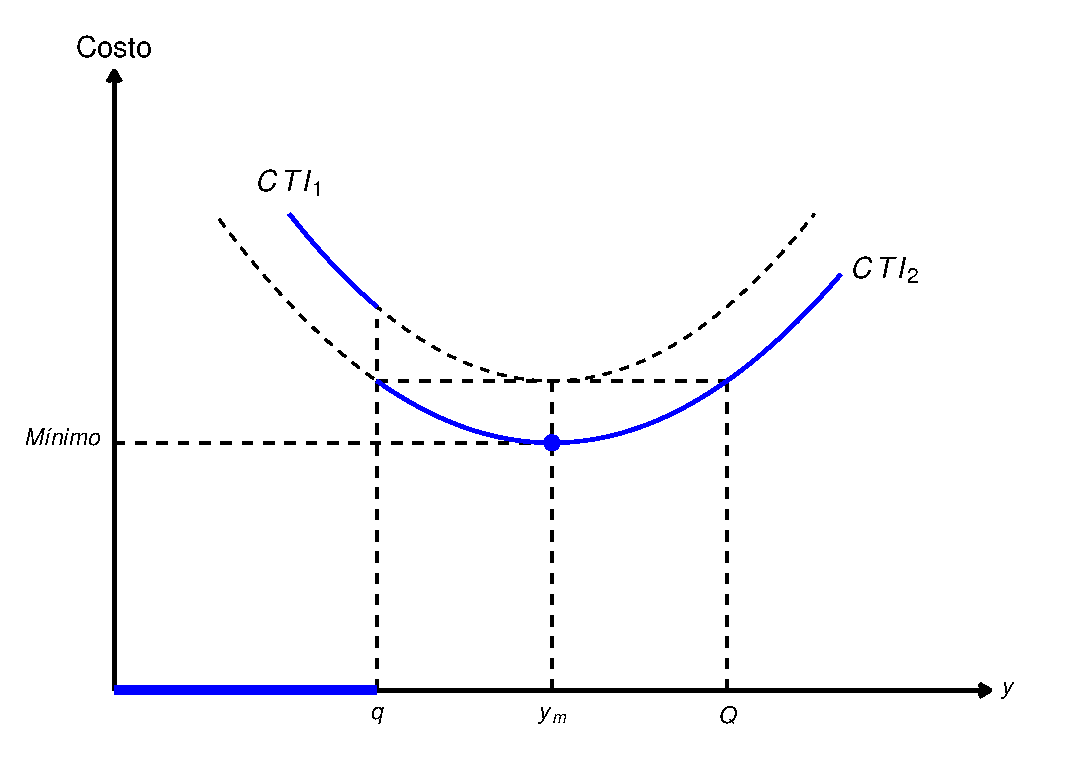
\includegraphics[width=13cm, height=6.1cm]{images/img4.pdf}
        \label{fig:img4a}
    \end{subfigure}

    \vspace{0.2cm}

    \begin{subfigure}[b]{1\textwidth}
    		\caption{\textbf{Caso 2:} ($q$) queda dentro de la zona II, $y^* = q$}
        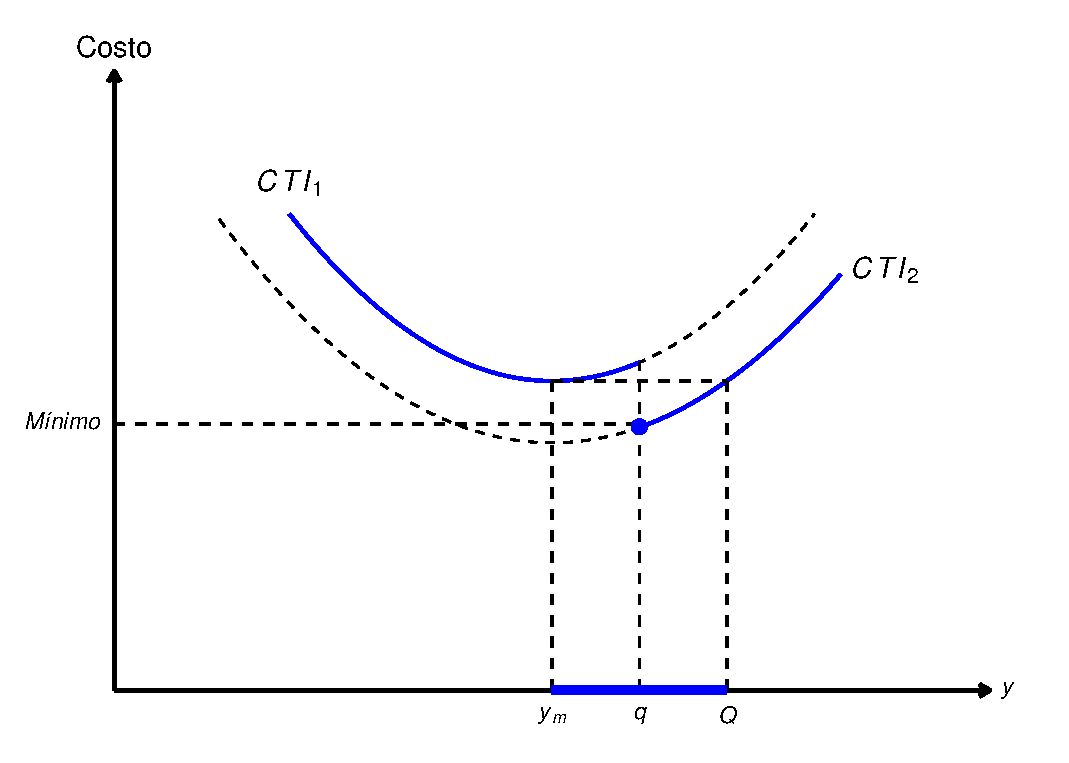
\includegraphics[width=13cm, height=6.1cm]{images/img5.pdf}
        \label{fig:img4b}
    \end{subfigure}
    
    % Salto de línea
    \vspace{0.2cm}
    
    % Segunda fila con una imagen centrada
    \begin{subfigure}[b]{1\textwidth} % Ancho mayor para la tercera imagen
        \caption{\textbf{Caso 3:} ($q$) queda dentro de la zona III, $y^* = y_m$}
        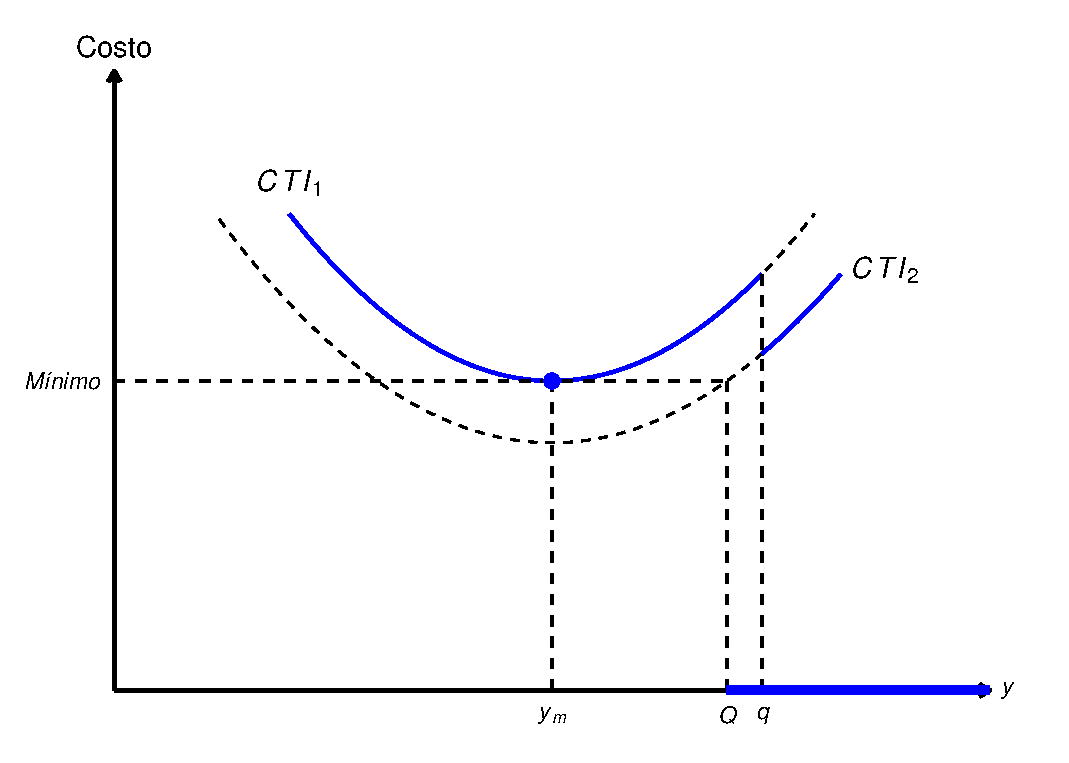
\includegraphics[width=13cm, height=6.1cm]{images/img6.pdf}
        \label{fig:img4c}
    \end{subfigure}
    \label{fig:img4}
\end{figure}

\newpage
\manualsubsubsection{2.2.15.3}{Modelo clásico de cantidad económica de pedido (EOQ) de varios productos con limitación de almacén}
En este modelo se considera que cada producto sigue el comportamiento del modelo clásico (EOQ) sin faltantes que se muestra en la Figura \ref{fig:img1}. Además se consideran que se tiene $n$ productos tal que $n>1$, entonces además de que los productos se utilizan con una demanda constante, a su vez tienen un espacio de almacenamiento con un límite de capacidad.

Definimos para cada producto $i$ tal que $i = 1, 2, \cdots , n$ sus respectivos
\begin{itemize}
	\item[$D_i=$] Tasa de demanda del producto $i$.
	\item[$K_i=$] Costo de preparación del producto $i$.
	\item[$h_i=$] Costo de retención del producto $i$.
	\item[$y_i=$] Cantidad de pedido del producto $i$.
	\item[$a_i=$] Espacio de almacenamiento para el producto $i$.
	\item[$A=$] Espacio de almacenamiento disponible para los $n$ productos.
\end{itemize}
Al igual que el modelo (EOQ) para cada producto $i$ en el que $i = 1, \cdots, n$ hallamos la duración del ciclo de pedido mediante la expresión (\ref{T}) quedando de la siguiente manera
\begin{equation}
	\label{T_i}
	{T}_{i} = \frac{y_i}{D_i}
\end{equation}
Cantidad de pedido óptima $y^*$ de la expresión (\ref{yopt}) para cada producto $i$
\begin{equation}
	\label{yiast}
	{y}_{i}^{*} = \sqrt{\frac{2{K}_{i}{D}_{i}}{{h}_{i}}}
\end{equation}
De igual forma para obtener el costo total de inventario $CTI(y)$ que se observa en la ecuación (\ref{CTI})
$$
CTI(y) = \frac{KD}{y} + DC + \frac{hy}{2}
$$
Para cada producto $i$ se borra el costo fijo $DC$ de donde $C$ es el costo por unidad del producto, ya que este no es el mismo al costo total al variar por producto, de tal forma que para cada producto el costo mínimo total quedaría de la siguiente forma:
\begin{equation}
	\label{CTI_i_opt}
	CTI({y}_{i}) = \frac{{K}_{i}{D}_{i}}{{y}_{i}} + \frac{{h}_{i}{y}_{i}}{2} 	
\end{equation} 
Y el costo mínimo total estaría dado por la siguiente función
\begin{eqnarray}
	CTI({y}_{1},{y}_{2},\cdots , {y}_{n}) &=& CTI({y}_{1}) + CTI({y}_{2}) + \cdots + CTI({y}_{n}) \nonumber \\
	 CTI({y}_{1},{y}_{2},\cdots , {y}_{n}) &=& \left(\frac{{K}_{1}{D}_{1}}{{y}_{1}} + \frac{{h}_{1}{y}_{1}}{2} 	 \right) + \left(\frac{{K}_{2}{D}_{2}}{{y}_{2}} + \frac{{h}_{2}{y}_{2}}{2} 	 \right) + \cdots + \left(\frac{{K}_{n}{D}_{n}}{{y}_{n}} + \frac{{h}_{n}{y}_{n}}{2} 	 \right) \nonumber \\
	 CTI({y}_{1},{y}_{2},\cdots , {y}_{n}) &=& \sum\limits_{i = 1}^{n} \left(\frac{{K}_{i}{D}_{i}}{{y}_{i}} + \frac{{h}_{i}{y}_{i}}{2} \right)
\end{eqnarray}
Tomando en cuenta de que el modelo no va a tener faltantes, el modelo matemático que exprese el inventario vendría a ser
$$
	\textsl{Minimizar }CTI({y}_{1},{y}_{2},\cdots , {y}_{n}) = \sum\limits_{i = 1}^{n} \left(\frac{{K}_{i}{D}_{i}}{{y}_{i}} + \frac{{h}_{i}{y}_{i}}{2} \right)
$$
Sujeto a
$$
\sum\limits_{i = 1}^{n} {a}_{i} {y}_{i} \leq A
$$
$$
{y}_{i} > 0, i = 1, 2, \cdots , n
$$
Primeramente se debe abordar el caso no restringido
$$
{y}_{i}^{*} = \sqrt{\frac{2{K}_{i}{D}_{i}}{{h}_{i}}}, i = 1, 2, \cdots , n
$$
Si la solución satisface la restricción, entonces el proceso termina. Caso contrario la restricción debe ser activada, uno de los métodos de activación es el método clásico de Lagrange (\ref{Mult_Lagrange}). Entonces el lagrangiano de la función es:
\begin{eqnarray}
	\label{funcion_lagrange}
	L(\lambda, {y}_{1}, {y}_{2}, \cdots , {y}_{n}) &=& CTI({y}_{1}, {y}_{2}, \cdots , {y}_{n}) - \lambda \left( \sum\limits_{i = 1}^{n} {a}_{i} {y}_{i} - A \right) \nonumber \\
	L(\lambda, {y}_{1}, {y}_{2}, \cdots , {y}_{n}) &=& \sum\limits_{i = 1}^{n} \left(\frac{{K}_{i}{D}_{i}}{{y}_{i}} + \frac{{h}_{i}{y}_{i}}{2} \right) - \lambda \left( \sum\limits_{i = 1}^{n} {a}_{i} {y}_{i} - A \right)
\end{eqnarray}
En donde $\lambda < 0$ es el multiplicador de Lagrange, asimismo la función de Lagrange es convexa, los valores óptimos de $y_i$ y $\lambda$ que minimizan a (\ref{funcion_lagrange}) se determina resolviendo el sistema
\begin{eqnarray}
	\label{lagran_yi}
	\frac{\partial L}{\partial {y}_{i}} = \frac{\partial}{\partial {y}_{i}} \left[ \sum\limits_{i = 1}^{n} \left(\frac{{K}_{i}{D}_{i}}{{y}_{i}} + \frac{{h}_{i}{y}_{i}}{2} \right) - \lambda \left( \sum\limits_{i = 1}^{n} {a}_{i} {y}_{i} - A \right) \right] = 0 \\
	\label{lagran_lambda}
	\frac{\partial L}{\partial \lambda} = \frac{\partial}{\partial \lambda} \left[ \sum\limits_{i = 1}^{n} \left(\frac{{K}_{i}{D}_{i}}{{y}_{i}} + \frac{{h}_{i}{y}_{i}}{2} \right) - \lambda \left( \sum\limits_{i = 1}^{n} {a}_{i} {y}_{i} - A \right) \right] = 0
\end{eqnarray}
De lo que resolviendo la primera derivada parcial (\ref{lagran_yi}) se tiene la siguiente expresión
\begin{eqnarray}
	\frac{\partial L}{\partial {y}_{i}} &=& - \frac{{K}_{i} {D}_{i}}{{y}_{i}^2} + \frac{{h}_{i}}{2} - \lambda {a}_{i} \nonumber
\end{eqnarray}
Esta expresión igualamos a cero y hallamos la cantidad de pedido óptimo ${y}_{i}^{*}$
\begin{eqnarray}
	\label{yi_opt_ast}
	- \frac{{K}_{i} {D}_{i}}{{y}_{i}^2} + \frac{{h}_{i}}{2} - \lambda {a}_{i} &=& 0 \nonumber \\
	\frac{{K}_{i} {D}_{i}}{{y}_{i}^2} &=& \frac{{h}_{i}}{2} - \lambda {a}_{i} \nonumber \\
	\frac{{K}_{i} {D}_{i}}{{y}_{i}^2} &=& \frac{{h}_{i} - 2 \lambda {a}_{i}}{2} \nonumber \\
	2 {K}_{i} {D}_{i} &=& {y}_{i}^{2} ({h}_{i} - 2 \lambda {a}_{i}) \nonumber \\
	{y}_{i}^{2} &=& \frac{2 {K}_{i} {D}_{i}}{{h}_{i} - 2 \lambda {a}_{i}} \nonumber \\
	{y}_{i} &=& \pm \sqrt{\frac{2 {K}_{i} {D}_{i}}{{h}_{i} - 2 \lambda {a}_{i}}} \quad \text{(solo se considera la parte positiva)} \nonumber \\
	{y}_{i}^{*} &=& \sqrt{\frac{2 {K}_{i} {D}_{i}}{{h}_{i} - 2 \lambda {a}_{i}}}
\end{eqnarray}
De igual forma resolviendo la derivada parcial (\ref{lagran_lambda}) se tiene la siguiente expresión
\begin{eqnarray}
	\frac{\partial L}{\partial \lambda} &=& A - \sum\limits_{i = 1}^{n} {a}_{i} {y}_{i} \nonumber
\end{eqnarray}
Ahora igualando a cero y reemplazando ${y}_{i}$ por el valor de ${y}_{i}^{*}$ de (\ref{yi_opt_ast}) se tiene
\begin{eqnarray}
	\label{lagran_lambda2}
	A - \sum\limits_{i = 1}^{n} {a}_{i} {y}_{i} &=& 0 \nonumber \\
	A - \sum\limits_{i = 1}^{n} {a}_{i} \sqrt{\frac{2 {K}_{i} {D}_{i}}{{h}_{i} - 2 \lambda {a}_{i}}} &=& 0 
\end{eqnarray}
Si $\lambda = 0$ en la expresión (\ref{yi_opt_ast}) se tiene la cantidad de pedido óptima $y^*$ igual a (\ref{yiast}), por lo que se debe tener un valor de $\lambda < 0$ para que cumpla la igualdad de (\ref{lagran_lambda2}) si no es así se vuelve a repetir el proceso asignando otro valor negativo $\lambda$ hasta lograr una aproximación a la igualdad (\ref{lagran_lambda2}).

\manualsubsubsection{2.2.15.4}{Modelo clásico de cantidad económica de pedido (EOQ) con escasez}\label{EOQ_escasez}
Uno de los problemas más grandes que se tienen en los modelos de inventarios son los faltantes, que es cuando la demanda no se satisface y genera retrasos, esto es debido a que el inventario agoto los productos en existencia hasta volver a reabastecerse, los casos en donde se permiten estos faltantes es cuando el cliente acepta este retraso si es necesario, donde se toma el riesgo de la pérdida del cliente o la caída del negocio. Este modelo toma en consideración estos casos extendiendo el modelo clásico (EOQ) que se observa en la Figura \ref{fig:img1} donde:
\begin{itemize}
	\item[$S=$] Nivel del inventario después de recibir $y$ unidades.
	\item[$y-S=$] Escasez del inventario antes de recibir $y$ unidades.
	\item[$t_1=$] Intervalo de tiempo en el cual el inventario no es negativo y satisface la demanda.
	\item[$t_2=$] Intervalo de tiempo en el cual el inventario es negativo y no satisface la demanda.
\end{itemize}
El comportamiento del modelo clásico de cantidad económica de pedido con escasez se observa en la Figura \ref{fig:imga}.
\newpage
\begin{figure}[H]
  \caption{Modelo clásico económica de pedido (EOQ) con demanda diferida}
  {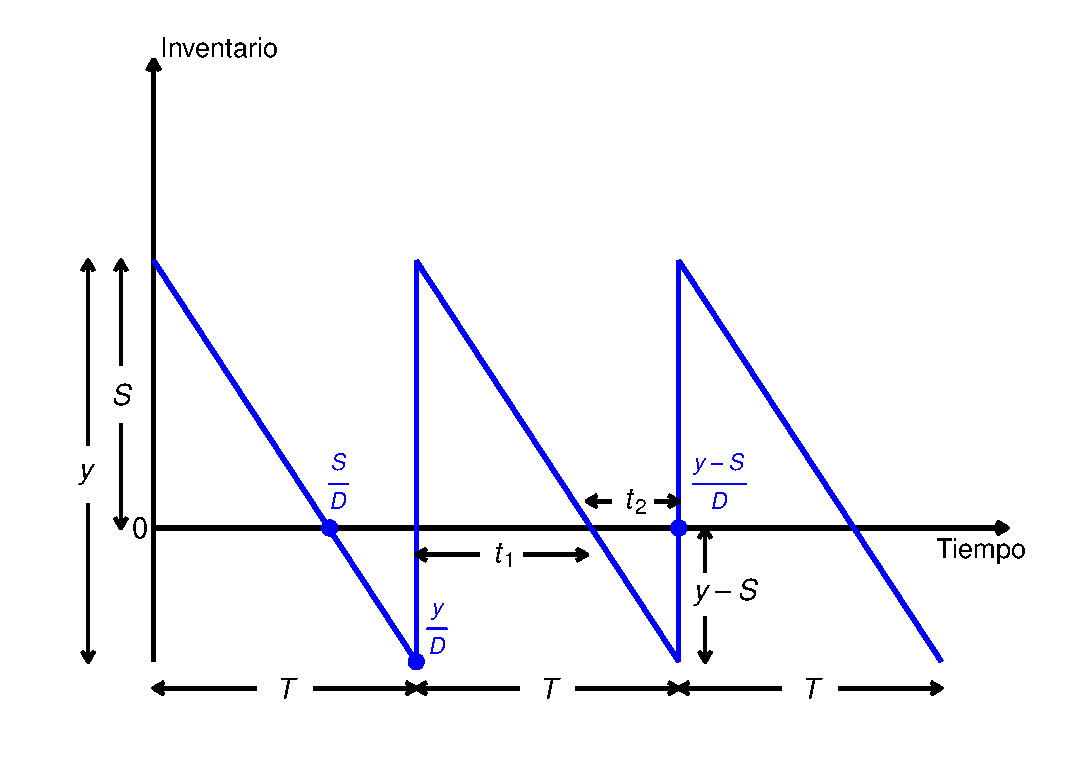
\includegraphics[width=15cm, height=7.7cm]{images/imga.pdf}}
  \label{fig:imga}
\end{figure}
En la cual por semejanza de triángulos podemos hallar el intervalo de tiempo que satisface la demanda:
\begin{eqnarray}
	\frac{t_1}{T} &=& \frac{S}{y} \nonumber \\
	t_1 &=& \frac{S}{y}T \nonumber
\end{eqnarray}
A esta expresión reemplazemos el valor $T$ de (\ref{T})
\begin{eqnarray}
	t_1 &=& \frac{S}{y} \left( \frac{y}{D} \right) \nonumber \\
	t_1 &=& \frac{S}{D}
\end{eqnarray}
De igual forma por semejanza de triángulos hallamos el intervalo en donde no se satisface la demanda:
\begin{eqnarray}
	\frac{t_2}{T} &=& \frac{y-S}{y} \nonumber \\
	t_2 &=& \frac{y-S}{y}(T) \nonumber
\end{eqnarray}
\newpage
\noindent De la misma forma reemplazamos $T$ de (\ref{T})
\begin{eqnarray}
	t_2 &=& \frac{y-S}{y} \left( \frac{y}{D} \right) \nonumber \\
	t_2 &=& \frac{y-S}{D}
\end{eqnarray}
Como se vieron en los anteriores casos para sacar el costo total del inventario $CTI(y)$ se tienen que tomar en cuenta el costo por producción en el intervalo de tiempo ($CPT$) enunciada en la expresión (\ref{CPT}). El costo de almacenamiento por intervalo de tiempo $(CAIT)$ se da solo en el tiempo $\frac{S}{D}$ por lo que extendiendo la expresión (\ref{CAIT}) reemplazando ``$y$'' por $S$ se tiene la siguiente expresión
\begin{equation}
	\label{CAITescasez}
	CAIT = \frac{hS^2}{2D}
\end{equation}
Ahora el déficit del inventario ocurre en un intervalo de tiempo $\frac{y-S}{D}$ en donde se tiene un costo de escasez ``$p$'', de la misma analogía que (\ref{CAIT}) se tiene la siguiente expresión para el costo de escasez por intervalo de tiempo $(CET)$
\begin{equation}
	\label{CETescasez}
	CET = \frac{p{(y-S)}^{2}}{2D} 	
\end{equation} 
De lo que el costo total por intervalo de tiempo $(CTT)$ estaría en función de la adición del costo de almacenamiento $(CAIT)$, el costo de producción $(CPT)$ y el costo por escasez $(CET)$ por intervalo de tiempo
\begin{equation}
	CTT = CPT + CAIT + CET
\end{equation}
Reemplazando los valores $(CPT)$, $(CAIT)$ y $(CET)$ por las expresiones (\ref{CPT}), (\ref{CAITescasez}) y (\ref{CETescasez}) respectivamente se tiene la siguiente expresión
\begin{equation}
	CTT = K + Cy + \frac{hS^2}{2D} + \frac{p{(y-S)}^{2}}{2D}
\end{equation}
De la misma forma que se realizó en (\ref{CTIdejado}) dividimos el $(CTT)$ por el tiempo $(T)$, y reemplazando $T$ por la expresión (\ref{T}), se tiene el costo total del inventario del modelo con demanda diferida.
\begin{eqnarray}
	\label{CTIy_esc_fal}
	CTI(y) &=& \frac{CTT}{T} \nonumber \\
	CTI(y) &=& \frac{K + Cy + \frac{hS^2}{2D} + \frac{p{(y-S)}^{2}}{2D}}{T} \nonumber \\
	CTI(y) &=& \frac{K + Cy + \frac{hS^2}{2D} + \frac{p{(y-S)}^{2}}{2D}}{\frac{y}{D}} \nonumber \\
%\end{eqnarray}
%\begin{eqnarray}
	CTI(y) &=& \frac{\frac{2DK + 2DCy + hS^2 + p{(y-S)}^{2}}{2D}}{\frac{y}{D}} \nonumber \\
	CTI(y) &=& \frac{2DK + 2DCy + hS^2 + p{(y-S)}^{2}}{2y} \nonumber \\
	CTI(y) &=& \frac{DK}{y} + DC + \frac{hS^2}{2y}+\frac{p{(y-S)}^{2}}{2y}
\end{eqnarray}
Para este caso en la expresión (\ref{CTIy_esc_fal}) se tienen dos variables de decisión ``$S$'' y ``$y$'', en lo cual para encontrar los valores óptimos $S^*$ y $y^*$ se halla el vector gradiente $\nabla CTI(y)$ con las respectivas derivadas parciales e igualando a cero, teniendo el siguiente sistema
\begin{eqnarray}
	\label{part1}
	\frac{\partial CTI(y)}{\partial S} &=& \frac{\partial}{\partial S} \left[ \frac{DK}{y} + DC + \frac{hS^2}{2y}+\frac{p{(y-S)}^{2}}{2y} \right] = 0 \\
	\label{part2}
	\frac{\partial CTI(y)}{\partial y} &=& \frac{\partial}{\partial y} \left[ \frac{DK}{y} + DC + \frac{hS^2}{2y}+\frac{p{(y-S)}^{2}}{2y} \right] = 0
\end{eqnarray}
Resolviendo (\ref{part1}) se tiene que:
\begin{eqnarray}
	\label{2_40}
	\frac{\partial CTI(y)}{\partial S} &=& \frac{\partial}{\partial S} \left[ \frac{DK}{y} + DC + \frac{hS^2}{2y}+\frac{p{(y-S)}^{2}}{2y} \right] \nonumber \\
	\frac{\partial CTI(y)}{\partial S} &=& \frac{2hS}{2y} + \frac{2p(y-S)(-1)}{2y} \nonumber \\
	\frac{\partial CTI(y)}{\partial S} &=& \frac{hS}{y} - \frac{p(y-S)}{y}
\end{eqnarray}
Ahora igualando (\ref{2_40}) a cero se tiene el valor para $S$ 
\begin{eqnarray}
	\label{S_240}
	\frac{hS}{y} - \frac{p(y-S)}{y} &=& 0 \nonumber \\
	\frac{hS - p (y-S)}{y} &=& 0 \nonumber \\
	hS &=& p(y-S) \nonumber \\
	hS &=& py - pS \nonumber \\
	hS + pS &=& py \nonumber \\
	S(h+p) &=& py \nonumber \\
	S &=& \frac{py}{h+p}
\end{eqnarray}
De la misma forma resolviendo (\ref{part2}) se tiene que:
\begin{eqnarray}
	\label{2_41}
	\frac{\partial CTI(y)}{\partial y} &=& \frac{\partial}{\partial y} \left[ \frac{DK}{y} + DC + \frac{hS^2}{2y}+\frac{p{(y-S)}^{2}}{2y} \right] \nonumber \\
	\frac{\partial CTI(y)}{\partial y} &=& - \frac{DK}{y^2} - \frac{hS^2}{2y^2} + \frac{2y[2p(y-S)]-[p{(y-S)}^{2}]2}{4y^2} \nonumber \\
	\frac{\partial CTI(y)}{\partial y} &=& - \frac{DK}{y^2} - \frac{hS^2}{2y^2} + \frac{4py(y-S)-2p{(y-S)}^{2}}{4y^2} \nonumber \\
	\frac{\partial CTI(y)}{\partial y} &=& - \frac{DK}{y^2} - \frac{hS^2}{2y^2} + \frac{2p(y-S)(2y-(y-S))}{4y^2} \nonumber \\
	\frac{\partial CTI(y)}{\partial y} &=& - \frac{DK}{y^2} - \frac{hS^2}{2y^2} + \frac{2p(y-S)(y+S)}{4y^2} \nonumber \\
	\frac{\partial CTI(y)}{\partial y} &=& - \frac{DK}{y^2} - \frac{hS^2}{2y^2} + \frac{p(y^2 - S^2)}{2y^2} \nonumber \\
	\frac{\partial CTI(y)}{\partial y} &=& - \frac{DK}{y^2} - \frac{hS^2}{2y^2} + \frac{py^2 - pS^2}{2y^2} \nonumber \\
	\frac{\partial CTI(y)}{\partial y} &=& - \frac{DK}{y^2} - \frac{hS^2}{2y^2} + \frac{py^2}{2y^2} - \frac{pS^2}{2y^2} \nonumber \\
	\frac{\partial CTI(y)}{\partial y} &=& - \frac{DK}{y^2} + \frac{p}{2} - \frac{hS^2}{2y^2} - \frac{pS^2}{2y^2} \nonumber \\
	\frac{\partial CTI(y)}{\partial y} &=& - \frac{DK}{y^2} + \frac{p}{2} - \frac{(h + p)}{2y^2}S^2
\end{eqnarray}
Ahora igualando (\ref{2_41}) a cero y reemplazando $S$ por el valor de (\ref{S_240})  se tiene el valor para la cantidad de pedido óptima $y^*$
\newpage
\begin{eqnarray}
		\label{y_ast}
	 	- \frac{DK}{y^2} + \frac{p}{2} - \frac{(h + p)}{2y^2}S^2 &=& 0 \nonumber \\
	 	- \frac{DK}{y^2} + \frac{p}{2} - \frac{(h + p)}{2y^2} {\left(\frac{py}{h+p} \right)}^{2} &=& 0 \nonumber \\
	 	- \frac{DK}{y^2} + \frac{p}{2} - \frac{p^2}{2(h+p)} &=& 0 \nonumber \\
	 	- \frac{DK}{y^2} + \frac{p(h+p)-p^2}{2(h+p)} &=& 0 \nonumber \\
	 	- \frac{DK}{y^2} + \frac{ph}{2(h+p)} &=& 0 \nonumber \\
	 	y^2 &=& \frac{2(h+p)DK}{ph} \nonumber \\
	 	y^2 &=& \left( \frac{2DK}{h} \right) \left( \frac{h+p}{p} \right) \nonumber \\
	 	y &=& \pm \sqrt{\left( \frac{2DK}{h} \right) \left( \frac{h+p}{p} \right)} \quad \text{(solo se considera la parte positiva)} \nonumber \\
	 	y^* &=& \sqrt{\frac{2DK}{h}} \sqrt{\frac{h+p}{p}}
\end{eqnarray}
De la misma forma reemplazamos $y^*$ de (\ref{y_ast}) en (\ref{S_240}) para obtener el nivel de inventario óptimo $(S^*)$ para recibir las cantidades de pedido óptimas.
\begin{eqnarray}
	\label{S_ast}
	S^* &=& \frac{py^*}{h+p} \nonumber \\
	S^* &=& \left(\frac{p}{h+p} \right) \sqrt{\frac{2DK}{h}} \sqrt{\frac{h+p}{p}} \nonumber \\
	S^* &=& \sqrt{\frac{(p^2)(2DK)(h+p)}{{(h+p)}^{2}hp}} \nonumber \\
	S^* &=& \sqrt{\frac{2DKp}{h(h+p)}} \nonumber \\
	S^* &=& \sqrt{\frac{2DK}{h}}\sqrt{\frac{p}{h+p}}
\end{eqnarray}
El tiempo de ciclo en cada pedido óptimo $(T^*)$ estaría expresado en base a (\ref{T}) reemplanzando por el valor de $y$ por $y^*$ de (\ref{y_ast})
\newpage
\begin{eqnarray}
	T^* &=& \frac{y^*}{D} \nonumber \\
	T^* &=& \frac{1}{D} \sqrt{\frac{2DK}{h}} \sqrt{\frac{h+p}{p}} \nonumber \\
	T^* &=& \sqrt{\frac{2DK(h+p)}{D^2 hp}} \nonumber \\
	T^* &=& \sqrt{\frac{2K}{Dh}} \sqrt{\frac{(h+p)}{p}}
\end{eqnarray}
La escasez del inventario óptima $(y^* - S^*)$ antes de recibir las $y^*$ unidades estaría en función de reemplazar $y$ por (\ref{y_ast}) y $S$ por (\ref{S_ast})
\begin{eqnarray}
	y^* - S^* &=& \sqrt{\frac{2DK}{h}} \sqrt{\frac{h+p}{p}} - \sqrt{\frac{2DK}{h}}\sqrt{\frac{p}{h+p}} \nonumber \\
	y^* - S^* &=& \sqrt{\frac{2DK}{h}} \left( \sqrt{\frac{h+p}{p}} - \sqrt{\frac{p}{h+p}} \right) \nonumber \\
	y^* - S^* &=& \sqrt{\frac{2DK}{h}} \left( \frac{{(\sqrt{h+p})}^{2} - {(\sqrt{p})}^{2}}{\sqrt{p(h+p)}}  \right) \nonumber \\
	y^* - S^* &=& \sqrt{\frac{2DK}{h}} \left( \frac{h}{\sqrt{p(h+p)}}  \right) \nonumber \\
	y^* - S^* &=& \sqrt{\frac{2DKh^2}{hp(h+p)}} \nonumber \\
	y^* - S^* &=& \sqrt{\frac{2DK}{p}} \sqrt{\frac{h}{(h+p)}}
\end{eqnarray}
Por último, de igual forma hallemos el total de inventario de la expresión (\ref{CTIy_esc_fal})
\begin{eqnarray}
	\label{CTI_escasezz}
	CTI(y) &=& \frac{DK}{y} + DC + \frac{hS^2}{2y}+\frac{p{(y-S)}^{2}}{2y} \nonumber \\
	CTI(y) &=& \frac{2DK + hS^2 + p{(y-S)}^{2}}{2y} + DC \nonumber \\
	CTI(y) &=& \frac{2DK + hS^2 + py^2 - 2pyS + pS^2}{2y} + DC \nonumber \\
	CTI(y^*) &=& \frac{2DK + (h+p){S}^{2} + p{y}^{2} - 2pyS}{2y} + DC
\end{eqnarray}
A la expresión reemplazemos los valores de $y$ y $S$ por los valores de $y^*$ y $S^*$ de las expresiones (\ref{y_ast}) y (\ref{S_ast}) respectivamente en la expresiòn (\ref{CTI_escasezz}) para hallar el costo mínimo total del inventario $CTI(y^*)$
\begin{eqnarray}
	CTI(y^*) &=& \frac{2DK + (h+p){S^*}^{2} + p{y^*}^{2} - 2py^*S^*}{2y^*} + DC \nonumber \\
	CTI(y^*) &=& \frac{2DK + (h+p){\left( \sqrt{\frac{2DK}{h}}\sqrt{\frac{p}{h+p}} \right)}^{2} + p{\left( \sqrt{\frac{2DK}{h}} \sqrt{\frac{h+p}{p}} \right)}^{2} - 2p\left( \sqrt{\frac{2DK}{h}} \sqrt{\frac{h+p}{p}} \right) \left( \sqrt{\frac{2DK}{h}}\sqrt{\frac{p}{h+p}} \right)}{2\left( \sqrt{\frac{2DK}{h}} \sqrt{\frac{h+p}{p}} \right)} + DC \nonumber \\
	CTI(y^*) &=& \frac{2DK + (h+p)\left( \frac{2DKp}{h(h+p)} \right) + p \left( \frac{2DK(h+p)}{hp} \right) - 2p \left( \sqrt{\frac{p{(2DK)}^{2}(h+p)}{h^2 p (h+p)}} \right) }{2 \left(\sqrt{\frac{2DK(h+p)}{hp}} \right)} + DC \nonumber \\
	CTI(y^*) &=& \frac{2DK + \frac{2DKp}{h}  + \frac{2DK(h+p)}{h} - 2p \left( \frac{2DK}{h} \right) }{2 \left(\sqrt{\frac{2DK(h+p)}{hp}} \right)} + DC \nonumber \\
	CTI(y^*) &=& \frac{2 \left( DK + \frac{DKp}{h}  + \frac{DK(h+p)}{h} - \frac{2DKp}{h} \right) }{2 \left(\sqrt{\frac{2DK(h+p)}{hp}} \right)} + DC \nonumber \\
	CTI(y^*) &=& \frac{\frac{DKh + DKp + DKh + DKp - 2DKp}{h}}{\sqrt{\frac{2DK(h+p)}{hp}}} + DC \nonumber \\
	CTI(y^*) &=& \frac{\frac{2DKh}{h}}{\sqrt{\frac{2DK(h+p)}{hp}}} + DC \nonumber \\
	CTI(y^*) &=& \sqrt{\frac{4D^2 K^2 h^2 hp}{h^2 2DK (h+p)}} + DC \nonumber \\
	CTI(y^*) &=& \sqrt{\frac{2DKhp}{h+p}} + DC \nonumber \\
	CTI(y^*) &=& \sqrt{2DKh} \sqrt{\frac{p}{h+p}} + DC
\end{eqnarray}
De la misma forma que se realizó en (\ref{yopt}) para demostrar que el valor es mínimo se realiza la prueba de la segunda derivada a la expresión del costo total de inventario $CTI(y)$ con respecto a ``$y$'' y ``$S$''
\newpage
\begin{eqnarray}
	\label{minimo2}
	\frac{d^2 CTI(y)}{dy^2} &=& \frac{d^2}{dy^2} \left[ \frac{DK}{y} + DC + \frac{hS^2}{2y}+\frac{p{(y-S)}^{2}}{2y} \right] \nonumber \\
	\frac{d^2 CTI(y)}{dy^2} &=& \frac{d}{dy} \left( - \frac{DK}{y^2} + \frac{p}{2} - \frac{(h + p)}{2y^2}S^2 \right) \nonumber \\
	\frac{d^2 CTI(y)}{dy^2} &=& \frac{2KD + (h+p)S^2}{y^3} \geq 0; \quad \forall y \\
	\frac{d^2 CTI(y)}{dS^2} &=& \frac{d^2}{dS^2} \left[ \frac{DK}{y} + DC + \frac{hS^2}{2y}+\frac{p{(y-S)}^{2}}{2y} \right] \nonumber \\
	\frac{d^2 CTI(S)}{dS^2} &=& \frac{d}{dS} \left( \frac{hS}{y} - \frac{p(y-S)}{y} \right) \nonumber \\
	\frac{d^2 CTI(S)}{dS^2} &=& \frac{h+p}{y} \geq 0; \quad \forall S
\end{eqnarray}
%Y de la misma forma que se realizó en (\ref{convexo1}) del teorema (\ref{convexo_dos_derivadas}) se demuestra la convexidad puesto que
%\begin{equation}
%	\label{convexo2}
%	\frac{d^2 CTI(y)}{dy^2} = \frac{2KD + (h+p)S^2}{y^3} < 0; \quad \forall y > 0
%\end{equation}
%La función $CTI(y)$ es convexa en $(0, + \infty)$, por lo que $y^*$ es el minimo de la función.
%--------------------------------------------
%----------- MODELOS PROBABILISTICOS ---------
%--------------------------------------------
\subsection{Modelos de inventario probabilísticos o estocásticos}
A diferencia del modelo determinístico presentado en la sección anterior, en este tipo de modelos se analizan los inventarios con un desconocimiento sobre la demanda para los periodos siguientes, aunque estos pueden ser representados como una variable aleatoria que siga una distribución de probabilidad conocida. \citep{taha2012investigacion}

Primeramente se explicarán los modelos con revisión continua que tienen dos modelos, la versión probabilística del modelo clásico (EOQ) y el modelo (EOQ) probabilizado que tiene una demanda aleatoria. Seguidamente se explicarán los modelos de revisión periódica como los modelos de un periodo sin costo de preparación, con costo de preparación y los modelos de varios periodos. 
\manualsubsubsection{2.2.16.1}{Modelo probabilizado de cantidad económica de pedido}\label{EOQ_probabilizado}
Son algunos los profesionales que buscaron la forma de adaptar el modelo EOQ determinístico para explicar de manera aproximada la naturaleza probabilística de la demanda. Se tiene un problema de periodo crítico en el ciclo del inventario entre la colocación y recepción de pedidos que pueda ocasionar que no se tengan los productos. Por lo que se toma la idea de tener la probabilidad de tener pocos faltantes y mayores reservas. Donde se tienen las siguientes variables:
\begin{itemize}
	\item[$B=$] Cantidad de la existencia de reserva.
	\item[$L=$] Tiempo de espera entre la llegada del producto y su siguiente colocación.
	\item[${x}_{L}=$] Variable aleatoria de la demanda durante el tiempo de espera $L$.
	\item[${\mu}_{L}=$] Media de la demanda en el tiempo de espera $L$.
	\item[${\sigma}_{L}=$] Desviación estándar de la demanda en el tiempo de espera $L$.
	\item[${y}^{*}=$] Cantidad de pedido óptimo del modelo (EOQ).
	\item[$\alpha =$] Probabilidad máxima de admitir faltantes durante el tiempo de espera $L$.
	\item[$B + {\mu}_{L} =$] Punto de pedido según la media de la demanda y la cantidad de reserva.
\end{itemize}
La relación del modelo EOQ con respecto a las reservas se muestran en la Figura \ref{fig:EOQ_ext}.

\begin{figure}[H]
  \caption{Modelo clásico EOQ con existencias de reservas $B$}
  {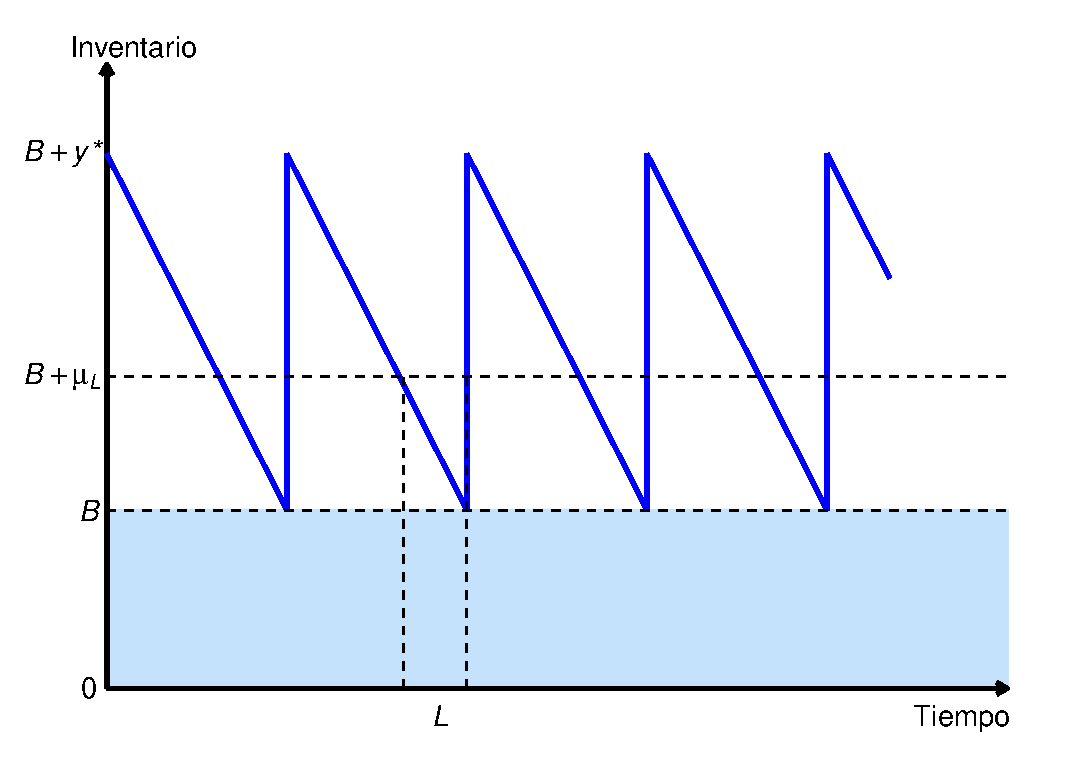
\includegraphics[width=15cm, height=8.5cm]{images/EOQ_ext.pdf}}
  \label{fig:EOQ_ext}
\end{figure} 

La hipótesis planteada del modelo es que la demanda por unidad de tiempo sigue una distribución normal con media $D$ y desviación estándar $\sigma$, denotado como $N(D,\sigma)$. Generalizando la definición de distribución normal mostrado en la subsección (\ref{Dist_normal}) expresando la demanda como una variable aleatoria durante un tiempo de espera $L$, en lo cual debe seguir la distribución de probabilidad normal con media ${\mu}_{L} = DL$ y desviación estándar ${\sigma}_{L} = \sqrt{L {\sigma}^{2}}$, representado de la siguiente manera ${x}_{L} \sim N({\mu}_{L},{\sigma}_{L})$. La definición de $L$ es la misma del modelo clásico en (\ref{Modelo_clas_EOQ}).
La cantidad de existencia de reservas $B$ se determina mediante la probabilidad de faltantes durante $L$ sea a lo máximo $\alpha$ de la siguiente forma:
\begin{equation}
	\label{eq:Prob1}
	P[ {x}_{L} \geq B + {\mu}_{L} ] \leq \alpha
\end{equation}
De lo cual a la expresión (\ref{eq:Prob1}) si despejamos con respecto a $B$ y estandarizamos se tiene la siguiente expresión:
\begin{eqnarray}
	\label{eq:Prob2}
	P[ {x}_{L} - {\mu}_{L} \geq B  ] &\leq& \alpha \nonumber \\
	P \left[ \frac{{x}_{L} - {\mu}_{L}}{{\sigma}_{L}} \geq \frac{B}{{\sigma}_{L}} \right] &\leq& \alpha \nonumber \\
	P \left[ z \geq \frac{B}{{\sigma}_{L}} \right] &\leq& \alpha 
\end{eqnarray}
De (\ref{eq:Prob2}) se tiene que $z = \frac{{x}_{L} - {\mu}_{L}}{{\sigma}_{L}}$ es la estandarización de ${x}_{L}$ que sigue una distribución normal estándar $N(0,1)$. Se define el parámetro ${K}_{\alpha}$ para la distribución normal estándar de modo que $P[z \geq {k}_{\alpha}] \leq \alpha$ que se observa en la Figura \ref{fig:img10}.
\begin{figure}[H]
  \caption{Probabilidad de que se agoten las reservas $P[z \leq {K}_{\alpha}] = \alpha$}
  {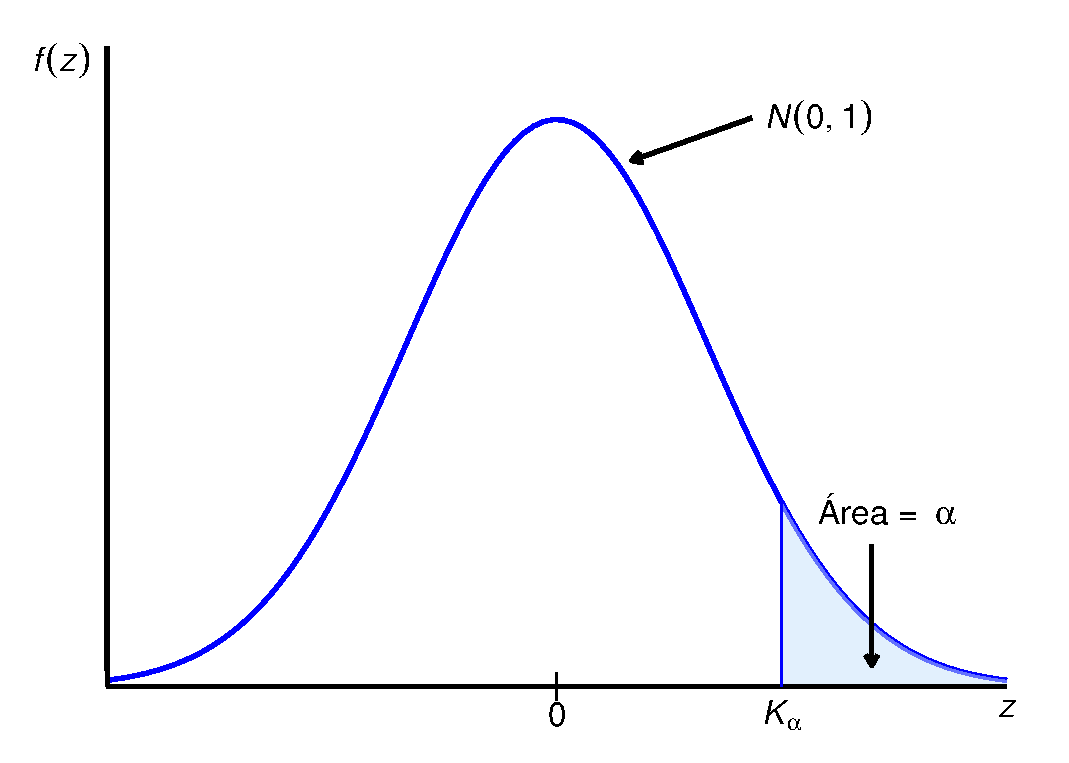
\includegraphics[width=15cm, height=7cm]{images/img10.pdf}}
  \label{fig:img10}
\end{figure} 
Por lo que el tamaño de reserva debe satisfacer la siguiente desigualdad
\newpage
\begin{equation}
	\label{eq:Prob3}
	B \leq {\sigma}_{L} {K}_{\alpha}
\end{equation}
En el cual de (\ref{eq:Prob3}) se tiene que ${\sigma}_{L}{K}_{\alpha}$ proporciona el valor mínimo de $B$ y se requiere que $L$ sea un valor entero ya sea por el valor exacto o redondeando el valor.

\manualsubsubsection{2.2.16.2}{Modelo cantidad de pedido económica (EOQ) probabilístico}
El modelo probabilizado EOQ visto en la anterior sección no hace verosimil la producción de una política óptima, ya que se ignora el hecho de que la demanda tenga un comportamiento probabilístico. Por lo cual el modelo de cantidad de pedido económica (EOQ) probabilístico toma en cuenta el comportamiento probabilístico de la demanda. De igual forma la política del inventario establece en realizar el pedido de ``$y$'' cantidades cuando el inventario llegue al punto de reorden ``$R$'' que al igual que en el modelo determinístico tiene un tiempo entre el pedido y la recepción del pedido. Para encontrar los valores óptimos de ``$y$'' y ``$R$'' se debe minimizar la suma esperada de los costos de retención y los costos de faltantes por unidad de tiempo. El modelo toma en cuenta tres suposiciones:
\begin{enumerate}
	\item La demanda que no se satisface en el ciclo de espera se guardan o almacenan.
	\item No se debe permitir más de un pedido pendiente.
	\item La distribución de la demanda en el ciclo de espera es estacionaria con el tiempo.
\end{enumerate}
Asimismo la función de costo total por unidad de tiempo se toman en cuenta las siguientes variables:
\begin{itemize}
	\item[$f(x) =$] Función de densidad de probabilidad de la demanda ``$x$'' durante el ciclo de espera.
	\item[$D =$] Demanda esperada por unidad de tiempo.
	\item[$h =$] Costo de retención o almacenamiento del inventario por unidad de tiempo.
	\item[$p =$] Costo por escasez o faltante del inventario.
	\item[$K =$] Costo de preparación del pedido.
\end{itemize}
El comportamiento del modelo se puede observar en la Figura \ref{fig:img11}.
\begin{figure}[h!]
  \caption{Modelo de inventario probabilístico con faltante}
  {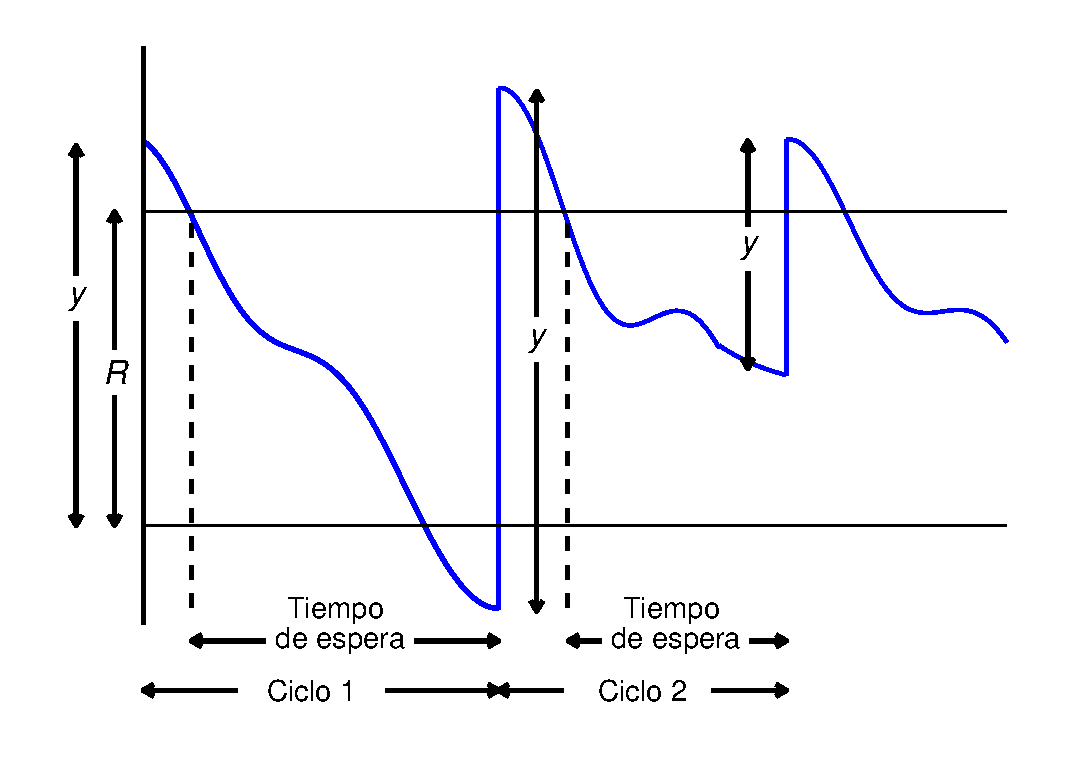
\includegraphics[width=15cm, height=7cm]{images/img11.pdf}}
  \label{fig:img11}
\end{figure} 
En el cual se observan que en los ciclos pueden ocurrir o no faltantes (tal vez con un comportamiento aleatorio), como en el ciclo 1 y 2 de la Figura \ref{fig:img11}. Con estas variables se determinan los elementos de la función de costos
\begin{enumerate}
	\item \textbf{Costo de preparación $(CPT)$:} Es la cantidad aproximada de pedidos por unidad de tiempo es $\frac{D}{y}$, de modo que el costo de preparación por unidad de tiempo es aproxidamente $\frac{KD}{y}$.
	\begin{equation}
		\label{prob:CPT}
		CPT = \frac{KD}{y}
	\end{equation}
	\item \textbf{Costo de retención esperado $(CRE)$:} Si $I$ es el nivel de inventario promedio, el costo de retención o almacenamiento pur unidad de tiempo es ``$hI$''. Para calcular $I$ se toma en cuenta el promedio de los inventarios esperados inicial y final de un ciclo es decir $y + E[R - x]$ y $E[R-x]$ respectivamente de la siguiente forma:
	\begin{eqnarray}
		\label{prob:I}
		I &=& \frac{(y + E[R-x])+E[R-x]}{2} \nonumber \\
		I &=& \frac{(y+E[R]-E[x])+E[R]-E[x]}{2} \nonumber \\
		I &=& \frac{y}{2} + 2\frac{(R-E[x])}{2} \nonumber \\
		I &=& \frac{y}{2} + R - E[x]
	\end{eqnarray}
	En el cual $R-E[x]$ se ignora que pueda ser negativo, ahora el costo de retención esperado $(CRE)$ estaría en función de $h$ e $I$ de la expresión (\ref{prob:I}) mediante la siguiente forma:
	\begin{eqnarray}
		\label{prob:CRE}
		CRE &=& hI \nonumber \\
		CRE &=& h \left( \frac{y}{2} + R - E[x] \right)
	\end{eqnarray}
	\item \textbf{Costo por faltanes esperado:} Los faltantes se dan en el caso que $x > R$. De lo cual tomando en cuenta una función de densidad (\ref{VAContinua}) su valor esperado en el ciclo se calcula como:
	\begin{equation}
		\label{prob:S}
		S = \int_{R}^{\infty} (x-R)f(x)dx
	\end{equation}
\end{enumerate}
Como el costo por escasez ``$p$'' es proporcional sólo a la cantidad faltante, el costo esperado por cada ciclo es $pS$ y tomando en cuenta $\frac{D}{y}$ ciclos por unidad de tiempo, el costo de escasez por unidad de tiempo $(CET)$ es:
\begin{eqnarray}
	\label{prob:CET}
	CET &=& \frac{pS}{T} \nonumber \\
	CET &=& \frac{pS}{\frac{y}{D}} \nonumber \\
	CET &=& \frac{pDS}{y}
\end{eqnarray}  
De lo cual el costo total del inventario $CTI$ es igual a la suma del costo de preparación $(CPT)$, costo de retención esperado $(CRE)$ y el costo de escasez $(CET)$ por unidad de tiempo de las expresiones (\ref{prob:CPT}), (\ref{prob:CRE}) y (\ref{prob:CET}) respectivamente. El cual estaría en función de ``$y$'' y ``$R$'' de la siguiente manera:
\begin{eqnarray}
	\label{prob:CTI_y_R}
	CTI(y,R) &=& CPT + CRE + CET \nonumber \\
	CTI(y,R) &=& \frac{DK}{y} + h \left( \frac{y}{2} + R - E[x] \right) + \frac{pDS}{y}
\end{eqnarray}
\newpage
Como se realizó antes las soluciones óptimas de $y^*$ y $R^*$ se determinan mediante las derivadas parciales e igualando a cero la expresión (\ref{prob:CTI_y_R}) mediante las siguientes ecuaciones:
\begin{eqnarray}
	\label{prob:CTI_y_der}
	\frac{\partial CTI(y,R)}{\partial y} &=& \frac{\partial}{\partial y} \left[\frac{DK}{y} + h \left(\frac{y}{2} + R - E[x] \right) + \frac{pDS}{y} \right] = 0 \\
	\label{prob:CTI_R_der}
	\frac{\partial CTI(y,R)}{\partial R} &=& \frac{\partial}{\partial R} \left[\frac{DK}{y} + h \left(\frac{y}{2} + R - E[x] \right) + \frac{pDS}{y} \right] = 0
\end{eqnarray}
De lo que resolviendo la primera derivada parcial (\ref{prob:CTI_y_der}) se tiene la siguiente expresión:
\begin{eqnarray}
	\frac{\partial CTI(y,R)}{\partial y} = - \frac{DK}{y^2} + \frac{h}{2} - \frac{pDS}{y^2} = 0 \nonumber
\end{eqnarray}
Esta expresión igualamos a cero y hallamos la cantidad de pedido óptima $y^*$
\begin{eqnarray}
	\label{prob:y_opt_int}
	- \frac{DK}{y^2} + \frac{h}{2} - \frac{pDS}{y^2} &=& 0 \nonumber \\
	-2DK + y^2 h - 2pDS &=& 0 \nonumber \\
	y^2 &=& \frac{2D(K + pS)}{h} \nonumber \\
	y &=& \pm \sqrt{\frac{2D(K+pS)}{h}} \quad \text{(solo se considera la parte positiva)} \nonumber \\
	y^* &=&  \sqrt{\frac{2D(K+pS)}{h}}
\end{eqnarray}
De la misma forma resolviendo (\ref{prob:CTI_R_der}) reemplazamos $S$ por la expresión (\ref{prob:S}) de lo cual se tiene
\begin{eqnarray}
	\frac{\partial CTI(y,R)}{\partial R} &=& \frac{\partial}{\partial R} \left[\frac{DK}{y} + h \left(\frac{y}{2} + R - E[x] \right) + \frac{pD}{y} \int_{R}^{\infty} (x-R)f(x)dx \right] \nonumber
\end{eqnarray}
Resolviendo la derivada parcial 
\begin{eqnarray}
	\frac{\partial CTI(y,R)}{\partial R} &=& h - \frac{pD}{y}\int_{R}^{\infty} f(x)dx \nonumber
\end{eqnarray}
Ahora igualando a cero
\begin{eqnarray}
	\label{prob:R_opt_int}
	h - \frac{pD}{y}\int_{R}^{\infty} f(x)dx &=& 0 \nonumber \\
	\int_{R}^{\infty} f(x)dx &=& \frac{hy^*}{pD}
\end{eqnarray}
De lo cual los valores óptimos de $y^*$ y $R^*$ no se hallan en formas cerradas, por lo que se usa un algoritmo númerico, desarrollado por Hadle y Whitin (1963) para hallar las soluciones a las ecuaciones (\ref{prob:y_opt_int}) y (\ref{prob:R_opt_int}).

El algoritmo converge en un número finito de iteraciones, siempre que se tenga una solución factible.

Si $R=0$ en las ecuaciones (\ref{prob:y_opt_int}) y (\ref{prob:R_opt_int}) se tiene los siguientes resultados:
\begin{eqnarray}
	\hat{y} &=& \sqrt{\frac{2D(K+pE[x])}{h}} \nonumber \\
	\tilde{y} &=& \frac{pD}{h} \nonumber
\end{eqnarray}
De lo cual los valores óptimos de ``$y$'' y ``$R$'' existen cuando $\tilde{y} \geq \hat{y}$. Si $S=0$ el valor mínimo de $y^*$ es $\sqrt{\frac{2KD}{h}}$. Los pasos del algoritmo son:
\begin{itemize}
	\item[\textbf{Paso 0:}] Use la solución inicial ${y}_{1} = y^* = \sqrt{\frac{2KD}{h}}$, y sea ${R}_{0} = 0$. Establezca $i = 1$ y continue al paso \textbf{i}.
	\item[\textbf{Paso i:}] Use ${y}_{i}$ para determinar ${R}_{i}$ a partir de la ecuación (\ref{prob:R_opt_int}). Si ${R}_{i} \approx {R}_{i-1}$ se detiene el proceso. La solución óptima es $y^* = y_{i}$ y $R^* = R_{i}$. Caso contrario use ${R}_{i}$ en la ecuación (\ref{prob:y_opt_int}) para calcular ${y}_{i}$. Establezca $i = i +1$ y repetir el paso $i$.
\end{itemize}

\manualsubsubsection{2.2.16.3}{Modelo de un periodo sin preparación}
Los modelos de un periodo para un artículo se da cuando se pide una sola vez para satisfacer la demanda del periodo. Cuando culmina el periodo los sobrantes se desechan. En este primer modelo no se tiene un costo de preparación al momento de colocar el pedido de lo cual se tienen las siguientes variables:
\begin{itemize}
	\item[$h=$] Costo de retención o almacenamiento del inventario en el periodo.
	\item[$p=$] Costo de escasez del inventario en el periodo.
	\item[$f(D)=$] Función de distribución de probabilidad de la demanda $(D)$ durante el periodo.
	\item[$y=$] Cantidad del pedido.
	\item[$x=$] Cantidad del inventario disponible antes del siguiente pedido.
\end{itemize}
De la misma manera que los anteriores modelos, el modelo determina el valor óptimo de ``$y$'' minimizando los costos de retención y faltantes. Si se tiene $y = y^*$ se tiene un óptimo en el cual la política de inventario exige pedir $y^* - x$ si $x < y$, caso contrario no se debe de realizar el pedido.

En este modelo sin preparación se relaciona con el almacenamiento como se observa en la Figura \ref{fig:img12}.
\begin{figure}[h!]
    \centering
    \caption{Modelo de inventario de un solo periodo con retención y escasez}
    
    \subfloat[(a)]{
        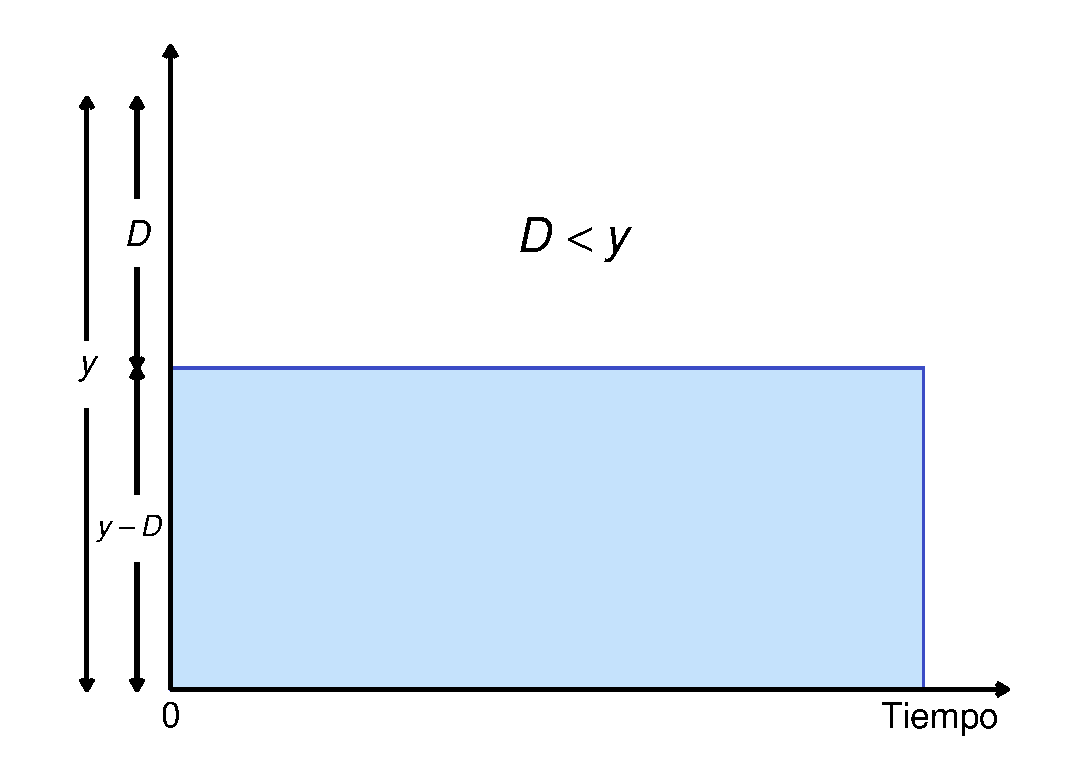
\includegraphics[width=0.48\textwidth,height=7cm]{images/img12.pdf}
        \label{fig:img12a}
    }
    \hfill
    \subfloat[(b)]{
        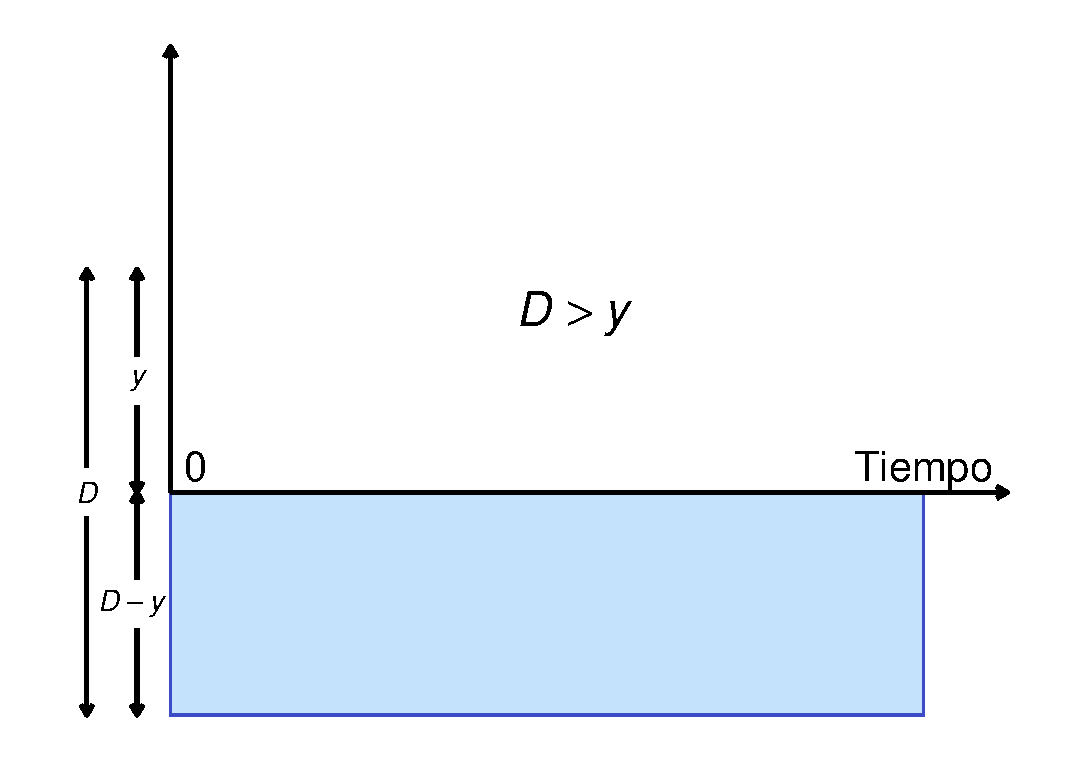
\includegraphics[width=0.48\textwidth,height=7cm]{images/img13.pdf}
        \label{fig:img12b}
    }

    \label{fig:img12}
\end{figure}

En el cual se tienen las siguientes suposiciones:
\begin{enumerate}
	\item En el momento que se recibe el pedido, la demanda empieza a ocurrir.
	\item No se tiene ningún costo de preparación. 
\end{enumerate}
De la Figura \ref{fig:img12} se tiene que si $D < y$, la cantidad sobrante $y-D$ se mantiene durante el periodo. Caso contrario si $D > y$ se tendrá una cantidad faltante $D-y$ durante el periodo.

Ahora el costo esperado durante el perido $E[C(y)]$ en función de la demanda estaría expresado para el caso discreto (\ref{VADiscreta}) y continuo (\ref{VAContinua}) teniendo las siguientes ecuaciones
\begin{eqnarray}
	\label{prob:un_periodo_con}
	E[C(y)] &=& h \int_{0}^{y} (y-D)f(D)dD + p \int_{y}^{\infty} (D-y)f(D)dD \quad \text{(caso continuo)} \\
	\label{prob:un_periodo_dis}
	E[C(y)] &=& h \sum\limits_{D = 0}^{y}(y-D)f(D) + p \sum\limits_{D = y+1}^{\infty} (D-y)f(D) \quad \text{(caso discreto)}
\end{eqnarray}
En lo cual se observa que $E[C(y)]$ en (\ref{prob:un_periodo_con}) y (\ref{prob:un_periodo_dis}) son convexos.

Para el caso continuo (\ref{prob:un_periodo_con}) como es convexo en ``$y$'' tiene un mínimo único. Tomando la primera derivada con respecto a ``$y$'' se tiene la siguiente expresión
\begin{eqnarray}
	\label{prob:der_E_con}
	\frac{d E[C(y)]}{dy} &=& \frac{d}{dy} \left[ h \int_{0}^{y} (y-D)f(D)dD + p \int_{y}^{\infty} (D-y)f(D)dD \right] \nonumber \\
	\frac{d E[C(y)]}{dy} &=& h \int_{0}^{y} f(D)dD - p \int_{0}^{\infty} f(D) dD
\end{eqnarray} 
Tomando en cuenta la segunda propiedad de la definición de variable aleatoria continua (\ref{VAContinua}), se puede realizar la siguiente expresión:
\begin{itemize}
 	\item $P[x \leq X] = \int_{0}^{X} f(x)dx$ 
 	\item $1 - P[x \leq X] = \int_{0}^{\infty} f(x)dx$
\end{itemize} 
Reemplazando en la expresión (\ref{prob:der_E_con}) se tiene la siguiente igualdad
\begin{eqnarray}
	\frac{d E[C(y)]}{dy} &=& hP[D \leq y] - p(1 - P[D \leq y]) \nonumber \\
	\frac{d E[C(y)]}{dy} &=& P[D \leq y] (h + p) - p \nonumber
\end{eqnarray}
E igualando a cero se tiene la siguiente igualdad:
\begin{eqnarray}
	\label{prob:P_D_men_y_opt}
	P[D \leq y] (h + p) - p &=& 0 \nonumber \\
	P[D \leq y^*] &=& \frac{p}{h+p}
\end{eqnarray}
Ahora para el caso discreto (\ref{prob:un_periodo_dis}) tomemos en cuenta las siguientes condiciones necesarias de optimalidad
\begin{itemize}
	\item $E[C(y-1)] \geq E[C(y)]$ y
	\item $E[C(y+1)] \geq E[C(y)]$ 
\end{itemize}
Que son suficientes ya que $E[C(y)]$ es una función convexa, empezemos hallando la expresiòn para $E[C(y+1)]$ en base a (\ref{prob:un_periodo_dis}) quedando de la siguiente manera
\begin{eqnarray}
	E[C(y+1)] &=& h \sum\limits_{D = 0}^{(y+1)}((y+1)-D)f(D) + p \sum\limits_{D = (y+1)+1}^{\infty} (D-(y+1))f(D) \nonumber \\
	E[C(y+1)] &=& h \left[ \sum\limits_{D = 0}^{y+1}(y+1)f(D) - \sum\limits_{D = 0}^{y+1}Df(D) \right] + \nonumber \\
	 & & p \left[ \sum\limits_{D = y+2}^{\infty} (D-y-1)f(D) \right] \nonumber \\
	E[C(y+1)] &=& h \left[ (y+1) \left( \sum\limits_{D = 0}^{y}f(D)+f(y+1) \right) - \left(\sum\limits_{D = 0}^{y} Df(D) + (y+1)f(y+1) \right) \right] + \nonumber \\
	 & & p \left[ \sum\limits_{D = y+1}^{\infty}(D-y-1)f(D)-( (y+1)-y-1 )f(y+1) \right] \nonumber \\
	 E[C(y+1)] &=& h \left[ (y+1) \sum\limits_{D = 0}^{y} f(D) + (y+1)f(y+1) - \sum\limits_{D = 0}^{y} Df(D) - (y+1)f(y+1) \right] + \nonumber \\
	  & & p \left[ \sum\limits_{D = y+1}^{\infty} (D-y-1)f(D) \right] \nonumber \\
	 E[C(y+1)] &=& h \left[ (y+1) \sum\limits_{D = 0}^{y} f(D) - \sum\limits_{D = 0}^{y} Df(D) \right] + \nonumber \\
	  & & p \left[ \sum\limits_{D = y+1}^{\infty} (D-y-1)f(D) \right] \nonumber \\
	E[C(y+1)] &=& h \left[ \sum\limits_{D = 0}^{y} (y+1-D) f(D) \right] + \nonumber \\
	  & & p \left[ \sum\limits_{D = y+1}^{\infty} (D-y-1)f(D) \right] \nonumber \\
	E[C(y+1)] &=& h \sum\limits_{D = 0}^{y}(y-D)f(D) + h \sum\limits_{D = 0}^{y}f(D) + p \sum\limits_{D = y+1}^{\infty}(D-y)f(D) - p \sum\limits_{D = y+1}^{\infty} f(D) \nonumber
\end{eqnarray}
\begin{eqnarray}
	\label{seguimos_res}
	E[C(y+1)] &=& h \sum\limits_{D = 0}^{y} (y-D) f(D) + p \sum\limits_{D = y+1}^{\infty} (D-y)f(D) + h \sum\limits_{D = 0}^{y} f(D) - p \sum\limits_{D = y+1}^{\infty} f(D) \nonumber \\
	E[C(y+1)] &=& E[C(y)] + h \sum\limits_{D = 0}^{y} f(D) - p \sum\limits_{D = y+1}^{\infty} f(D)
\end{eqnarray}
Por la segunda satisfacción de la definición (\ref{defn_vadisc}) de variable aleatoria discreta (\ref{VADiscreta}) se tiene la siguiente igualdad:
\begin{eqnarray}
	\sum\limits_{D = 0}^{y}f(D) + \sum\limits_{D = y+1}^{\infty} f(D) &=& 1 \nonumber \\
	\sum\limits_{D = y+1}^{\infty} f(D) &=& 1 - \sum\limits_{D = 0}^{y}f(D) \nonumber
\end{eqnarray}
Reemplazando esta igualdad en la expresión (\ref{seguimos_res}) obtenemos lo siguiente
\begin{eqnarray}
	\label{prob:Prim_cond_optima}
	E[C(y+1)] &=& E[C(y)] + h \sum\limits_{D = 0}^{y} f(D) - p \left(1 - \sum\limits_{D = 0}^{y}f(D) \right) \nonumber \\
	E[C(y+1)] - E[C(y)] &=& h \sum\limits_{D = 0}^{y} f(D) - p + p \sum\limits_{D = 0}^{y}f(D) \nonumber \\
	E[C(y+1)] - E[C(y)] &=& (h+p) \sum\limits_{D = 0}^{y}f(D)  - p \nonumber \\
	E[C(y+1)] - E[C(y)] &=& (h+p) P[D \leq y] - p
\end{eqnarray}
De la misma forma ahora hallando la expresiòn para $E[C(y-1)]$ en base a (\ref{prob:un_periodo_dis}) se tiene
\begin{eqnarray}
	E[C(y-1)] &=& h \sum\limits_{D = 0}^{(y-1)}((y-1)-D)f(D) + p \sum\limits_{D = (y-1)+1}^{\infty} (D-(y-1))f(D) \nonumber \\
	E[C(y-1)] &=& h \sum\limits_{D = 0}^{y-1}(y-D)f(D) - h \sum\limits_{D = 0}^{y-1}f(D) + p \sum\limits_{D = y}^{\infty} (D-y)f(D) + p \sum\limits_{D = y}^{\infty} f(D) \nonumber \\
	E[C(y-1)] &=& h \left[ \sum\limits_{D = 0}^{y}(y-D)f(D) - (y-y)f(y) \right] - h \sum\limits_{D = 0}^{y-1}f(D) \nonumber \\
	 & & + p \left[ \sum\limits_{D = y+1}^{\infty}(D-y)f(D) + (y-y)f(y) \right] + p \sum\limits_{D = y}^{\infty} f(D) \nonumber \\
	E[C(y-1)] &=& h \sum\limits_{D = 0}^{y}(y-D)f(D) - h \sum\limits_{D = 0}^{y-1}f(D) + p \sum\limits_{D = y+1}^{\infty} (D-y)f(D) + p \sum\limits_{D = y}^{\infty} f(D) \nonumber
\end{eqnarray}
\begin{eqnarray}
	\label{seguimos_res2}
	E[C(y-1)] &=& h \sum\limits_{D = 0}^{y}(y-D)f(D) + p \sum\limits_{D = y+1}^{\infty} (D-y)f(D) - h \sum\limits_{D = 0}^{y-1}f(D) + p \sum\limits_{D = y}^{\infty} f(D) \nonumber \\
	E[C(y-1)] &=& E[C(y)] - h \sum\limits_{D = 0}^{y-1}f(D) + p \sum\limits_{D = y}^{\infty} f(D)
\end{eqnarray}	
De la misma forma por la definición (\ref{defn_vadisc}) de variable aleatoria discreta (\ref{VADiscreta}) se tiene la siguiente igualdad:
\begin{eqnarray}
	\sum\limits_{D = 0}^{y-1}f(D) + \sum\limits_{D = y}^{\infty} f(D) &=& 1 \nonumber \\
	\sum\limits_{D = y}^{\infty} f(D) &=& 1 - \sum\limits_{D = 0}^{y-1}f(D) \nonumber
\end{eqnarray}
Reemplazando esta igualdad en la expresión (\ref{seguimos_res2}) obtenemos lo siguiente
\begin{eqnarray}
	\label{prob:Seg_cond_optima}
	E[C(y-1)] &=& E[C(y)] - h \sum\limits_{D = 0}^{y-1}f(D) + p \left( 1 - \sum\limits_{D = 0}^{y-1}f(D) \right) \nonumber \\
	E[C(y-1)] - E[C(y)] &=& - h \sum\limits_{D = 0}^{y-1}f(D) + p - p \sum\limits_{D = 0}^{y-1} f(D) \nonumber \\
	E[C(y-1)] - E[C(y)] &=& - (h+p) \sum\limits_{D = 0}^{y-1}f(D) + p \nonumber \\
	E[C(y-1)] - E[C(y)] &=& - (h+p) P[D \leq y-1] + p
\end{eqnarray}
En lo cual tomando la primera condición de optimalidad $E[C(y-1)] \geq E[C(y)]$ y reemplazando por los valores de (\ref{prob:Seg_cond_optima}) se tiene la siguiente desigualdad
\begin{eqnarray}
	\label{prob:seg_cond_des}
	E[C(y-1)] & \geq & E[C(y)] \nonumber \\
	E[C(y-1)] - E[C(y)] & \geq & 0 \nonumber \\
	- (h+p) P[D \leq y-1] + p & \geq & 0 \nonumber \\
	(h+p) P[D \leq y-1] - p & \leq & 0 \nonumber \\
	P[D \leq y-1] & \leq & \frac{p}{h+p}
\end{eqnarray}
Tomando la segunda condición de optimalidad $E[C(y+1)] \geq E[C(y)]$ y reemplazando por los valores de (\ref{prob:Prim_cond_optima}) se tiene la siguiente desigualdad
\begin{eqnarray}
	\label{prob:prim_cond_des}
	E[C(y+1)] & \geq & E[C(y)] \nonumber \\
	E[C(y+1)] - E[C(y)] & \geq & 0 \nonumber \\
	(h+s) P[D \leq y] - p & \geq & 0 \nonumber \\
	P[D \leq y] & \geq & \frac{p}{h+p}
\end{eqnarray}
Ahora tomando las expresiones (\ref{prob:seg_cond_des}) y (\ref{prob:prim_cond_des}) se tiene la siguiente desigualdad
\begin{equation}
	P[D \leq y^* - 1] \leq \frac{p}{h+p} \leq P[D \leq y^*]
\end{equation}

\manualsubsubsection{2.2.16.4}{Modelo de un periodo con costos de preparación}
Siendo igual que el modelo anterior de un periodo sin costos de preparación, en este modelo se incide el costo de preparación denotado por $K$. Entonces tomando en cuenta la expresión (\ref{prob:un_periodo_con}) y le adjuntamos el costo de preparación, se tiene la siguiente expresión para el costo esperado durante el periodo $E[\bar{C}(y)]$:
\begin{eqnarray}
	E[\bar{C}(y)] &=& K + E[C(y)] \nonumber \\
	E[\bar{C}(y)] &=& K + h \int_{0}^{y} (y-D)f(D)dD + p \int_{y}^{\infty} (D-y)f(D)dD
\end{eqnarray}
De la misma manera el valor óptimo $y^*$ de la expresión (\ref{prob:P_D_men_y_opt}) se debe satisfacer lo siguiente
\begin{equation}
	P[y \leq y^*] = \frac{p}{h+p}
\end{equation}
Tomando a $K$ como una constante el valor mínimo de $E[\bar{C}(y)]$ ocurre también en $y^*$. La política de pedido óptima se observa en la Figura \ref{fig:img14}.
\newpage
\begin{figure}[H]
  \caption{Política de pedido óptima (s-S) del modelo de un solo periodo con costo de preparación}
  {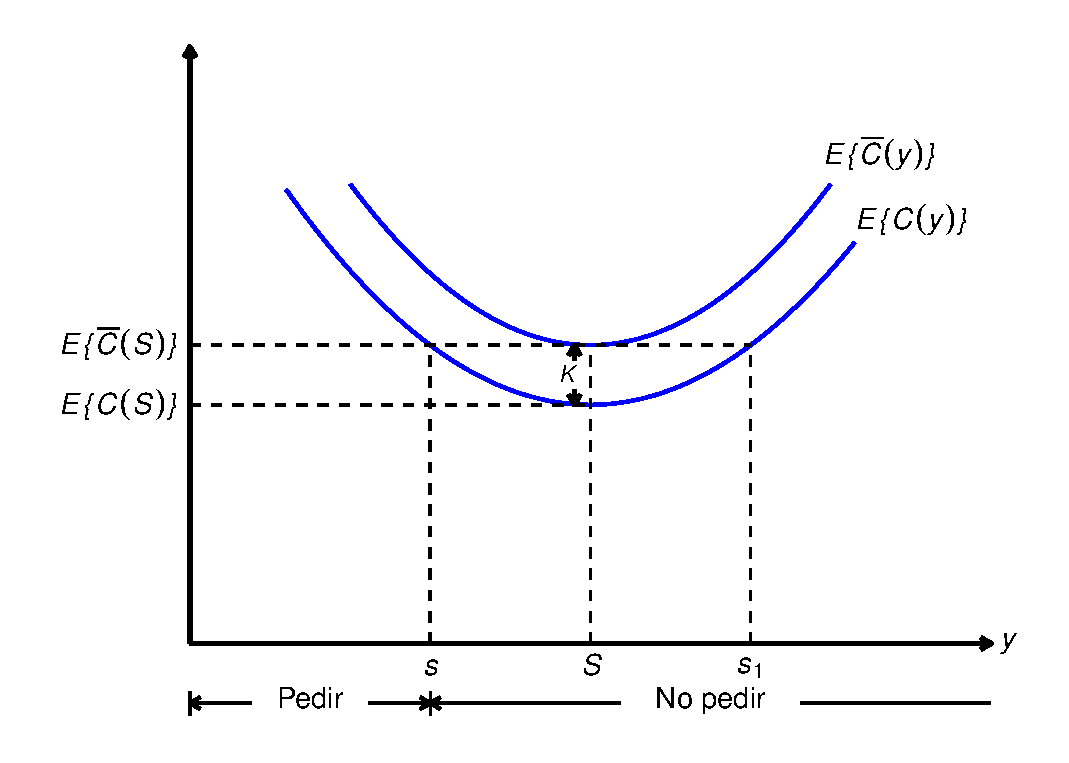
\includegraphics[width=13.5cm, height=7cm]{images/img14.pdf}}
  \label{fig:img14}
\end{figure}
En el cual se observa que si $S = y^*$ y el valor de $s < S$ se puede determinar mediante la siguiente ecuación:
\begin{eqnarray}
	E[C(s)] &=& E[\bar{C}(S)] \nonumber \\
	E[C(s)] &=& K + E[C(S)], \quad s < S
\end{eqnarray}
Si en la ecuación se tiene otro valor ${s}_{1} > S$ se le descarta. 

Entonces para la política de pedido suponemos que $x$ es la cantidad disponible antes de colocar el siguiente pedido, se tienen tres condiciones:
\begin{enumerate}
	\item $x < s$
	\item $s \leq x \leq S$
	\item $x > S$ 
\end{enumerate}

\begin{description}
    \item[\textbf{Caso 1 $(x > s)$:}] Como ya se tiene una cantidad $x$ en el cual su costo equivale a $E[C(x)]$. Si realizamos un pedido adicional $y-x$ donde $y > x$ su costo para $y$ estaría dado por $E[\bar{C}(y)]$ en el que se incluye el costo de preparación $K$. De la Figura \ref{fig:img14} se tiene
    $$
        \min_{y>x} E[\bar{C}(y)] = E[\bar{C}(S)] < E[C(x)]
    $$
    En el que la política de inventario óptima es pedir $S-x$ unidades.

    \item[\textbf{Caso 2 $(s \leq x \leq S)$:}] De la Figura \ref{fig:img14} se tiene
    $$
        E[C(x)] \leq \min_{y>x}E[\bar{C}(y)] = E[\bar{C}(S)]
    $$
    En el que la política de inventario indica que no se debería realizar el pedido para este caso. Por lo que $y^* = x$.

    \item[\textbf{Caso 3 $(x > S)$:}] De la Figura \ref{fig:img14} se tiene que $y > x$
    $$
        E[C(x)] < E[\bar{C}(y)]
    $$
    Al igual que en el caso 2, no se debería realizar el pedido o sea $y^* = x$.
\end{description}

Por lo que la política de inventario utiliza la \textsl{política s-S} que resume el pedido de la siguiente manera

\begin{equation}
	y^* =
	\left\{
	\begin{array}{ll}
		S-x & \text{si } x < s \\
		x, & \text{si } x \geq s
	\end{array}
	\right.
\end{equation}
En el cual se debe realizar el pedido $(S-x)$ si $x < s$ y no realizar el pedido si $x \geq s$, esta política esta garantizado ya que la función de costo es convexa.

\manualsubsubsection{2.2.16.5}{Modelo de varios periodos}
A diferencia de los dos anteriores modelos mencionados, en este modelo se presentan varios periodos bajo el supuesto de que no se tenga costo de preparación. Además se permite un retraso en el cumplimiento de la demanda y no se tiene un retraso en la entrega.

La demanda $D$ sigue una función de densidad $f(D)$ para cualquier periodo. Se tiene un factor de descuento $\alpha$ tal que $\alpha < 1$, por lo que la cantidad monetario disponible $A$ durante los $n$ periodos tendrán un valor de ${\alpha}^{n}A$. En el caso de que el inventario tenga $n$ periodos y que la escasez se deja pendiente en un periodo se define
\begin{itemize}
	\item[${F}_{i}({x}_{i}) =$] Utilidad máxima esperada durante los periodos $i, i+1, i+2, \cdots, n$ dado que ${x}_{i}$ es la cantidad disponible antes de colocar el siguiente pedido en el periodo $i$  
\end{itemize}
Teniendo en cuenta el costo e ingreso por unidad denotadas por $c$ y $r$ respectivamente, asimismo tomando las notaciones vistas en los modelos de un periodo y ${F}_{n+1}({y}_{n}-D)=0$ se tiene el siguiente modelo de programación probabilística.
\begin{align}
    F_{i}(x_{i}) &= \max_{y_{i} \geq x_{i}} 
    \left\{ -c({y}_{i}-{x}_{i}) + \int_{0}^{{y}_{i}} \left[ rD - h ({y}_{i}-D) \right] f(D) dD \right. \nonumber \\
    & \quad + \int_{{y}_{i}}^{\infty} \left[ r{y}_{i}+ \alpha r (D-{y}_{i}) - p(D-{y}_{i}) \right] f(D) dD \nonumber \\
    & \quad + \alpha \int_{0}^{\infty} F_{i+1}({y}_{i}-D) f(D) dD 
    \left. \vphantom{\int_{0}^{\infty}} \right\}, \quad \text{para } i = 1,2, \dots, n
\end{align}

El valor de ${x}_{i}$ puede ser negativa por la escasez pendiente, se incluye la cantidad $\alpha r (D-{y}_{i})$ en la segunda integral porque $(D - {y}_{i})$ es la demanda no satisfecha en el periodo $i$ que debe ser satisfecha en el periodo $i+1$. El problema se resuelve mediante la manera recursiva. Si la cantidad de pedidos en los periodos es finita, la ecuación recursiva se reduce a
\begin{align}
    F(x) &= \max_{y \geq x} 
    \left\{ -c(y-x) + \int_{0}^{y} \left[ rD - h (y-D) \right] f(D) dD \right. \nonumber \\
    & \quad + \int_{y}^{\infty} \left[ ry+ \alpha r (D-y) - p(D-y) \right] f(D) dD \nonumber \\
    & \quad + \alpha \int_{0}^{\infty} F(y-D) f(D) dD 
    \left. \vphantom{\int_{0}^{\infty}} \right\}
\end{align}
Donde ``$x$'' y ``$y$'' son los inventarios durante cada periodo antes y después de recibir el pedido respectivamente.

El valor óptimo de $y$ se determina a partir de la siguiente condición necesaria y suficiente ya que la función de ingreso $F(x)$ es cóncava
\newpage
\begin{align}
	\label{prob:alpha_der_partial}
    \frac{\partial F(x)}{\partial y}  &= \frac{\partial}{\partial y} 
    \left[ \max_{y \geq x} \left\{ -c(y-x) + \int_{0}^{y} \left[ rD - h (y-D) \right] f(D) dD \right. \right. \nonumber \\
    & \quad + \int_{y}^{\infty} \left[ ry+ \alpha r (D-y) - p(D-y) \right] f(D) dD \nonumber \\
    & \quad + \alpha \int_{0}^{\infty} F(y-D) f(D) dD 
    \left. \vphantom{\int_{0}^{\infty}} \right\} 
    \left. \vphantom{\int_{0}^{\infty}} \right] \nonumber \\
    \frac{\partial F(x)}{\partial y}  &= -c -h \int_{0}^{y}f(D)dD + \int_{y}^{\infty}[(1- \alpha )r + p]f(D)dD \nonumber \\
    & \quad + \alpha \int_{0}^{\infty} \frac{\partial F(y-D)}{\partial y}f(D)dD = 0
\end{align}

El valor de $\frac{\partial F(y-D)}{\partial y}$ se determina de la siguiente manera. Si hay más unidades $\beta > 0$ disponibles al inicio del siguiente periodo, la utilidad del siguiente periodo se incrementará en $c \beta$, ya que se pide esa cantidad de manera menor, lo que indica que:
$$
\frac{\partial F(y-D)}{\partial y}=c
$$
De lo que en (\ref{prob:alpha_der_partial}) la condición necesaria es
$$
-c-h \int_{0}^{y}f(D)dD+[(1-\alpha)r+p]\left( 1- \int_{0}^{y}f(D)dD \right) + \alpha c \int_{0}^{\infty}f(D)dD = 0
$$
Sea $w = \int_{0}^{y}f(D)dD$ y además se sabe que $\int_{0}^{\infty}f(D)dD=1$ por la definición de variable aleatoria continua ($\ref{VAContinua}$), reemplazando en la condición y resolviendo se tiene la siguiente expresión
\begin{eqnarray}
	-c-hw+[(1-\alpha)r+p](1-w)+\alpha c &=& 0 \nonumber \\
	-c-hw+[r-\alpha r + p](1-w)+ \alpha c &=& 0 \nonumber \\
	-c-wh+r-\alpha r + p - wr + w \alpha r - w p + \alpha c &=& 0 \nonumber \\
	wh + wr - w \alpha r + wp &=& -c+r - \alpha r + p + \alpha c \nonumber \\
	w (h+r- \alpha r + p) &=& p + r - \alpha r - c + \alpha c \nonumber \\
	w (p+h+r- \alpha r) &=& p + r(1 - \alpha) -c(1 - \alpha) \nonumber
\end{eqnarray}
\begin{eqnarray}
	w (p+h+r(1- \alpha)) &=& p + (r-c)(1 - \alpha) \nonumber \\
	w &=& \frac{p + (r-c)(1 - \alpha)}{p+h+r(1- \alpha)} \nonumber
\end{eqnarray}
Reemplazando $w = \int_{0}^{y}f(D)dD$ se tiene el nivel óptimo del inventario $y^*$ determinado a partir de
\begin{equation}
	\int_{0}^{y^*}f(D)dD = \frac{p + (r-c)(1 - \alpha)}{p+h+r(1- \alpha)}
\end{equation}
En el cual la política de inventario óptima durante cada periodo, si el nivel de inventario es $x$ se da de la siguiente manera
\begin{equation}
	y^* =
	\left\{
	\begin{array}{ll}
		y^* - x & \text{si } x < y^* \\
		x, & \text{si } x \geq y^*
	\end{array}
	\right.
\end{equation}
En el cual se debe realizar el pedido $({y}^{*}-x)$ si $x < y^*$ y no realizar el pedido si $x \geq y^*$.
%--------------------------------------------
%----------- ORGANIZACION DEL CSI   ---------
%--------------------------------------------
%\newpage
\subsection{Organización del centro de salud integral ``La Fuente''}

\subsubsection{Historia}
\textsl{LA FUENTE CENTRO DE SALUD INTEGRAL} es una Organización Cristiana que opera desde el año 2005 en el distrito de San Jerónimo, Cusco, Perú. Se constituye formalmente como Asociación Civil Sin Fines de Lucro el 28 de Octubre del año 2008.

Nuestro deseo es brindar atención excelente en servicios de salud a la población del Cusco y su alrededor, y, al hacerlo, compartir el amor que Dios nos ha mostrado a través de Jesucristo.

Nuestro equipo esta compuesto por médicos norteamericanos titulados en su especialidad respectiva, y profesionales peruanos debidamente licenciados. Hablamos inglés, castellano y quechua.

\subsubsection{Misión}
Promover vidas saludables para nuestros pacientes, brindándoles la mejor atención a nuestro alcance: preventiva de rehabilitación y curativa, de manera integral, atendiendo tanto su salud física como espiritual, sobre el fundamento de nuestra fe en Jesucristo.

\subsubsection{Visión}
Ser, al 2035 una organización lider en salud a nivel nacional, y referente en Oftalmología a nivel global, que muestre a Jesucristo en cada servicio que brindamos a todas las personas que lleguen a nosotros.

\subsubsection{Valores}

\begin{table}[H]
    \caption{Valores La Fuente Centro de Salud Integral}
    \begin{tabular}{p{2.65cm} p{5.5cm} p{6cm} } % Define anchos personalizados para cada columna
        \hline
        \textbf{VALORES CENTRALES} & \textbf{METAS} & \textbf{PRINCIPIOS} \\
        \hline
        \textbf{Compasión} & Atención con empatía & Amor y cuidado \\
        \hline
        \textbf{Justicia} & Acceso equitativo & Equidad / No discriminación \\
        \hline
        \textbf{Servicio} & Servicios de alta calidad & Diligencia \\
        \hline
        \textbf{Integridad} & Promoción de las mejores prácticas éticas y transparentes & Alineación con valores cristianos \\
        \hline
        \textbf{Cooperación} & Trabajo efectivo en equipo & Impacto mediante la colaboración \\
        \hline
    \end{tabular}
\end{table}

\subsubsection{Estructura organizativa}

\begin{enumerate}
	\item \textbf{ORGANO DE DIRECCIÓN}
	\begin{enumerate}
		\item Dirección General
	\end{enumerate}
	\item \textbf{ORGANOS DE ASESORAMIENTO}
	\begin{enumerate}
		\item Departamento Legal
		\item Departamento de Contabilidad y Finanzas
		\item Medicina Ocupacional
		\item Seguridad y Salud en el Trabajo
		\item INLASER (Marketing) 
	\end{enumerate}
	\item \textbf{ORGANOS DE APOYO}
	\begin{enumerate}
		\item Administración General
		\item Dirección de Operaciones
		\item Departamento de Logística de Insumos Médicos
		\begin{itemize}
			\item Cotizaciones
			\item Almacén 
		\end{itemize}
		\item Ingeniería Biomédica
		\item Infraestructura y Servicios Generales
		\begin{itemize}
			\item Portería y Seguridad
			\item Limpieza y mantenimiento 
		\end{itemize}
		\item Sistemas $\&$ TI
		\begin{itemize}
			\item Soporte Técnico
			\item Software y Programación 
		\end{itemize}
		\item Gestión de HHCC
	\end{enumerate}
	\item \textbf{ORGANOS EN LINEA}
	\begin{enumerate}
	 	\item UPSS Farmacia
	 	\item Departamento de Fisioterapia
	 	\begin{itemize}
	 		\item Admisión / Recepción
	 		\item Consultorios Externos 
	 	\end{itemize}
	 	\item Departamento de Odontología
	 	\begin{itemize}
	 		\item Admisión / Recepción
	 		\item Consultorios Externos 
	 	\end{itemize}
	 	\item Departamento de Oftalmología
	 	\begin{itemize}
	 		\item Área de Admisión
	 		\begin{itemize}
	 		 	\item Admisión
	 		 	\item Recepción
	 		 \end{itemize}
	 		 \item Área de Asistencia Técnica
	 		 \begin{itemize}
	 		  	\item Triaje
	 		  	\item Indicaciones
	 		  	\item Exámenes Especiales 
	 		  \end{itemize}
	 		  \item Optometría
	 		  \item Oftalmología
	 		  \item Especialidades
	 		  \begin{itemize}
	 		   	\item Retina
	 		   	\item Glaucoma
	 		   	\item Oculoplastía 
	 		   \end{itemize}
	 		  \item Sala de Cirugías y Procedimientos
	 		  \begin{itemize}
	 		   	\item Cotizaciones
	 		   	\item Esterilización
	 		   	\item Cirugías no electivas y Electivas 
	 		   \end{itemize}
	 		  \item Óptica
	 		  \begin{itemize}
	 		   	\item Asesoría de Ventas
	 		   	\item Laboratorio Óptico 
	 		   \end{itemize} 
	 	\end{itemize}
	 \end{enumerate} 
\end{enumerate}

\begin{landscape} % Iniciar la página en formato horizontal
\begin{figure}[h!]
  \caption{Organigrama La Fuente Centro de Salud Integral}
  {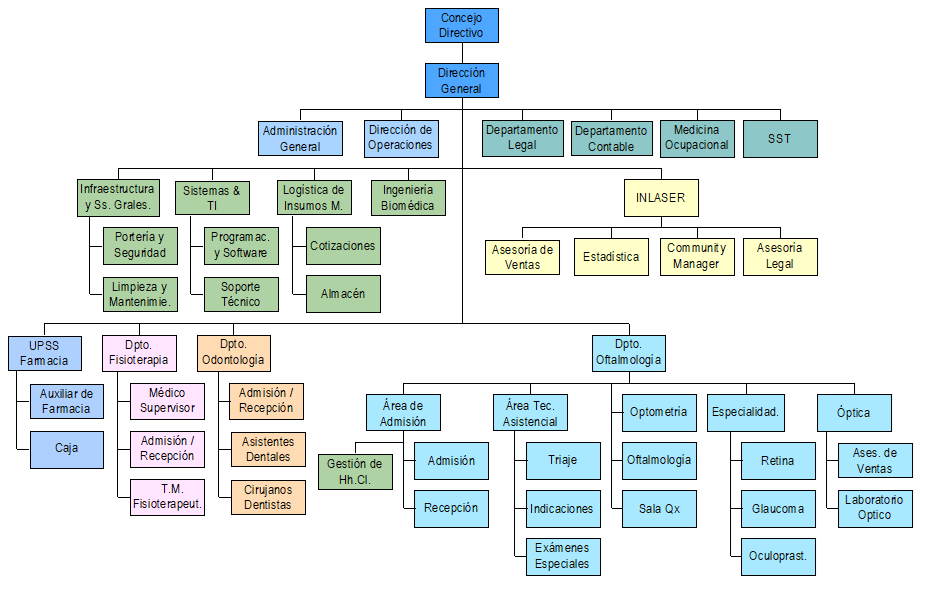
\includegraphics[width=25cm, height=14cm]{images/organigrama.png}}
  \label{fig:organigrama_fuente}
\end{figure} 
\end{landscape} % Finalizar la página horizontal

\section{Marco conceptual}
\noindent
\textbf{Análisis ABC:} Análisis que divide el inventario en tres grupos. El grupo A es más importante que el grupo B que, a su vez más importante que el C. \citep{render2006metodos}\vspace{0.25cm}

\noindent
\textbf{Inventario:} Es cualquier recurso almacenado que se utiliza para satisfacer una necesidad actual o futura. \citep{render2006metodos}\vspace{0.25cm}

\noindent
\textbf{Demanda:} Es la cantidad que los compradores desean adquirir o comprar de un determinado bien para satisfacer sus necesidades. \citep{mankiw2007principios}\vspace{0.25cm}

\noindent
\textbf{Costos:} Valor de mercado de los insumos que la empresa utiliza en la producción o mantenimiento del bien. Todo lo que el vendedor renuncia para producir el bien \citep{mankiw2007principios}\vspace{0.25cm}

\noindent
\textbf{Descuentos por cantidad:} Costo por unidad cuando se tienen grandes órdenes de un artículo. \citep{render2006metodos}\vspace{0.25cm}

\noindent
\textbf{Faltantes:} Situación que ocurre cuando no hay inventario en disponibilidad. \citep{render2006metodos}\vspace{0.25cm}

\noindent
\textbf{Punto de Reorden:} Momento en el que se toma la decisión de cuando realizar el pedido. \citep{taha2012investigacion}\vspace{0.25cm}

\noindent
\textbf{Tiempo de entrega:} Tiempo que se demora en recibir la orden una vez realizada. \citep{render2006metodos}






















